%!TEX root = ../template.tex
%%%%%%%%%%%%%%%%%%%%%%%%%%%%%%%%%%%%%%%%%%%%%%%%%%%%%%%%%%%%%%%%%%%%
%% chapter2.tex
%% NOVA thesis document file
%%
%% Chapter with the template manual
%%%%%%%%%%%%%%%%%%%%%%%%%%%%%%%%%%%%%%%%%%%%%%%%%%%%%%%%%%%%%%%%%%%%

\typeout{NT FILE chapter2.tex}%

\chapter{Time Series Fundamentals}
\label{cha:theory}

The content of this thesis is diverse and covers several different topics. Therefore, we will start by setting the foundations that are necessary to fully capture the essence of this work. For this, we introduce the concepts and topics covered, and provide the necessary definitions and corresponding notation used in this work. Let us begin by explaining global definitions related to \textit{time series}, which is the data type of interest in this work. Then, examples of \textit{time series}, in particular \textit{biosignals}, are given. Further, standard pre-processing methods, representation forms, and distance measures are also explained.
\par
Additionally, as this work makes a strong connection between time series and their textual nature, the association between text and time series is introduced in this chapter. Finally, we also explain the standard quantitative metrics used to show the results and validate the proposed methods.

\section{Global Definitions}
\label{sec:global}

The information gathered by sensors is a physical quantity that varies with time. These are called \textit{time series} and are the main topic of this work.\\\\
\textbf{Time Series:} A \textit{time series} is a sequence of real values ordered in time with length $n \in \mathbb{N}$: $T = (t_1, t_2, ..., t_n)$. A \textit{biosignal} is a category of \textit{time series}.
Several data domains rely on the \textit{multidimensional time series} acquisition from one sensor's multiple axes, such as an accelerometer's three directions, or multiple sources, such as an \gls{imu} that fuses three different sensors.\\\\
\textbf{Multidimensional Time Series:} A \textit{multidimensional time series} is a set of $k \in \mathbb{N}$ \textit{time series} belonging to the same acquisition: $\{T_1, T_2, ..., T_k\}$. Segments of interest, called \textit{subsequences}, are often searched inside a \textit{time series}.\\\\
\textbf{Subsequence:} A \textit{subsequence} is a segment of a (\textit{multidimensional}) \textit{time series} with size $w \in \mathbb{N}$, starting from a given position \textit{i} and ending at position \textit{i+w}. Therefore, two instants, defined as \textit{events}, delimit a \textit{subsequence} in time.\\\\
\textbf{Event:} An \textit{event} is an instant in time \textit{e} that indicates the presence of a relevant occurrence in the \textit{time series}. Multiple \textit{events} segment the time series into several \textit{subsequences} of different lengths. Hence, \textit{event} detection is often considered \textit{time series} segmentation or change point detection\cite{cpd_alan}. To be clear, we will use the terms \textit{event detection} and \textit{segmentation} when discussing our methods, but can eventually use the term change point detection when comparing with other methods. A common strategy used in time series data mining to find relevant \textit{subsequences} or \textit{events} is the \textit{moving window}.\\\\
\textbf{Moving Window:} A \textit{moving window} is a process of sliding along a time series $T$ to apply a specific method on each \textit{subsequence} it hovers, a common strategy used in \textit{time series} data mining to find relevant \textit{subsequences} and \textit{events}.
The window has, similar to the \textit{subsequence}, a predefined size $w \in \mathbb{N}$, which starts at a given position \textit{i} and ends at position \textit{i+w}.
The process of \textit{moving windows} is iterative, and windows can overlap each other. The next window will start at \textit{i+o}, where  \textit{o} $\in [1, w]$ is the overlapping size ($o=1$ for total overlap and $o=w$ for no overlap).
On each \textit{moving window} from each \textit{subsequence} of the (\textit{multidimensional}) \textit{time series}, features can be extracted to form a \textit{feature series}.

With a moving window, each \textit{subsequence} of a \textit{time series} can be filtered, features can be extracted or distances can be measured. We will show several utilities of this technique further when introducing methods used to pre-process a raw time series and apply standard distance measures. More importantly, we start by explaining the importance of a moving window to represent a \textit{time series} with a feature, a \textit{feature series}.\\\\
\textbf{Feature Series:} A \textit{feature series} is a feature representation of a time series with size $m = \frac{n}{w-o}$ that depends on the overlap size $o \in \mathbb{N}$ of the \textit{moving window}. In the case of a \textit{multidimensional time series}, the \textit{feature series} stack a \textit{multifeature series} with size $f_{k,m}$. Multiple features extracted from one dimension or various dimensions are grouped into a \textit{feature matrix}.\\\\\textbf{Feature Matrix ($F_M$):} A \textit{feature matrix} with size $r \times (k\times m)$, represents that each of the $k$ dimensions produces $r$ features. This \textit{feature matrix}, which characterizes the (\textit{multidimensional}) \textit{time series} in statistical, temporal or spectral domains, is used to compute the \textit{self-similarity matrix}.

Having introduced essential concepts for the understanding of the next few sections, we further give an overview of essential techniques used in time series processing and analysis, namely filtering methods, representation methods, distance measures and its applications, and a formal explanation of the relationship between text and \textit{time series}. 



%\textbf{Definition 1 - \gls{T}:} A \gls{T} is a sequence of real values ordered in time with length $n \in \mathbb{N}$: $T = (t_1, t_2, ..., t_n)$.
%    Several domains of data rely on the acquisition of multiple \gls{T} from multiple axes of the same sensor (e.g. the 3-axis accelerometer) or from multiple sources (e.g. IMU as a fusion of three different sensors), creating a \textit{multi-dimensional time series}.\\
%    
%\textbf{Definition 2 - \gls{MT}:} A \gls{MT} is a set of $k \in \mathbb{N}$ time series belonging to the same acquisition: $\{T_1, T_2, ..., T_k\}$. Segments of interest are often searched inside a \textit{time series}. A segment is called a \textit{subsequence}:\\
%    
%\textbf{Definition 3 - \gls{sT}:} A \gls{sT} is a segment of the time series with size $w \in \mathbb{N}$ and starting from a given position \textit{i} and ending at position \textit{i+w} from the \gls{T} or \gls{MT}. A \gls{sT} is delimited by two instants in time. This sample that segments a \gls{sT} can be considered an \textit{event}.\\
%    
%\textbf{Definition 4 - Event (E):} Following the definitions of \cite{event_def1, event_def2}, which state that "\textit{an event is a dynamic phenomenon whose behaviour changes enough over time to be considered a qualitatively significant change}" and "characterized by an interval of measurements that differs significantly from some underlying baseline", we consider that an \textit{event} is an instant in time \textit{e} that indicates the presence of a relevant occurrence in the time series. Multiple \textit{events} segment the time series into several \textit{subsequences} of different lengths. Therefore, \textit{event} detection is often considered time series segmentation or change point detection\cite{cpd_alan}. To be clear, we will use the terms \textit{event detection} and \textit{segmentation} when discussing our methods, but can eventually use the term change point detection when comparing with other methods.
%    
%
%
%\textbf{Definition 5 - Moving Window (MW):} A \textit{moving window} is a process of sliding along a time series $T$ to apply a specific method on each \textit{subsequence} it hovers. The window has, such as the \textit{subsequence}, a predefined size $w \in \mathbb{N}$, which starts at a given position \textit{i} and ends at position \textit{i+w}. The process is iterative and can be made overlapping windows or not. The next window will start at \textit{i+o}, being \textit{o} the overlapping size and \textit{o} $\in [1, w]$ ($1$ for total overlap and $w$ for no overlap).\\
%
%With a \textit{MW}, each \textit{subsequence} of a time series can be filtered, features can be extracted or distances can be measured. We will show several utilities of this technique further when introducing methods used to pre-process a raw time series and apply standard distance measures. Before explaining these strategies, we will give examples of time series covered in this work, focusing on \textit{biosignals}.



%\par
%Depending on the context and which conditions the data is gathered, the raw information can contain disturbances or should be transformed into another dimension to extract what matters. The set of tasks taken to prepare the \textit{time series} to enhance information retrieval is called \textit{pre-processing}. The pre-processing steps we will discuss involve filtering, normalization, and transformation.
%\par
%After preparing the data, information retrieval techniques are employed, which typically rely on distance measures. In that sense, the standard distance measures are explained. These distances will not only be performed on the numerical domain, but also on the text-domain. Therefore, an introduction to the \textit{textual abstraction} of time series will be made in this section as well.
%
%\section{Time Series Samples}
%\label{sec:ts_samples}
%
%(CHECK CATIA's THESIS)

\section{Filtering}
\label{sec:filt}

Time series have multiple sources of disturbance. This disturbance is usually called \textit{noise} and is defined as an unwanted form of energy, but it can have multiple interpretations. It can be caused by internal sources inside a device, such as \textit{white noise}, or be due to external sources, such as motion artifacts, wandering baseline, sensor detachment, or the magnetic field from surrounding devices. Any of these disturbances will affect the analysis stage and should be detected or removed.

\subsection{Spectral Filtering}
\label{subsec:spec_filt}

Several methods can be used to reduce the influence of noise in the analysis. Standard filtering methods, such as low-pass, band-pass, and high-pass filters can be used to reduce the presence of specific frequency bandwidths that are not relevant. There are many configurations for these types of filters, being one commonly used the \textit{Butterworth} filter, with the following frequency response:

\begin{equation}
H_{j\omega} = \frac{1}{\sqrt{1+\epsilon^2 \left(\frac{\omega}{\omega_c}\right)^2}},
\end{equation}

where $n$ is the order of the filter, $\omega$ the frequency ($\omega=2\pi f$), and $\epsilon$ the maximum amplitude gain. 


\subsection{Smoothing}
\label{subsec:smooth}

Another method, often used to reduce the presence of noise and is a variant of a low-pass filter, is the smoothing technique. Several variations of this method exist, being the simplest one a moving average, which uses a moving window to calculate the mean in each iteration. Other approaches also convolve the signal with a specific window ($H$) (e.g. \textit{Hanning window}), which instead of giving the same weights to all the samples of the moving window (moving average), attributes a higher weight to the moving window's central samples.
 
\begin{equation}
Tm_i = \Sigma_{j=a}^{a+w} T_jH_{j-a},
\end{equation}

where $Tm_i$ is the $i^{th}$ smoothed sample of the time series $T$, segmented by $a$ and $a+w$ ($w$ is the size of the moving window) and $H$ is the window function used to smooth the signal.

\subsection{Wandering Baseline}
\label{subsec:w_baseline}

Another type of disturbance on the data that is usually removed is a wandering baseline. An example typically occurs in \gls{ecg} signals, where the respiration creates a wandering baseline on it. This type of disturbance has a very low frequency compared to the meaningful information on the data and can be removed by subtracting a \textit{smoothed} version of the original data or applying a high pass filter.

\section{Normalization} 
\label{sec:normalize}

Normalization of data is an important step in any data mining process. It is essential for data standardization and scaling while keeping the morphology and shape of the time series. Several methods can be used for this purpose, namely:

\begin{equation}
\overline{T} = \frac{T}{max(|T|)},
\end{equation}

where the normalized signal ($\overline{T}$) is scaled by the absolute maximum of $T$. It is the simplest approach to normalization and guarantees that values are scaled linearly and their modulus cannot be higher than 1.
\par
A variation of this process is the normalization by the range of amplitudes:

\begin{equation}
\overline{T} = \frac{T-min(T)}{max(T)-min(T)},
\end{equation}

where the time series $T$ is normalized to range between [0,1].
Another normalization method, called \textit{z-normalization}, is very commonly used and relies on the distribution of its values:

\begin{equation}
\overline{T} = \frac{T-\mu_T}{\sigma_T},
\end{equation}

where the time series $T$ is subtracted by its mean, $\mu_T$ and scaled by its standard deviation, $\sigma_T$. The resulting values represent how many standard deviations the signal is away from the mean.

\section{Transformation} 
\label{sec:transform}

In information retrieval, data has often to be re-scaled, simplified, approximate, or represented into another data type. Each can contribute in their way to capture the most relevant and meaningful information, or discover a new type of information that once was hidden in the original data. Dozens of methods exist for time series representation, such as \gls{svd} or wavelet transform, but only the ones relevant to this thesis will be explained.

\subsection{Spectral Transformation}
\label{subsec:spec_transform}

\begin{figure}
    \centering
    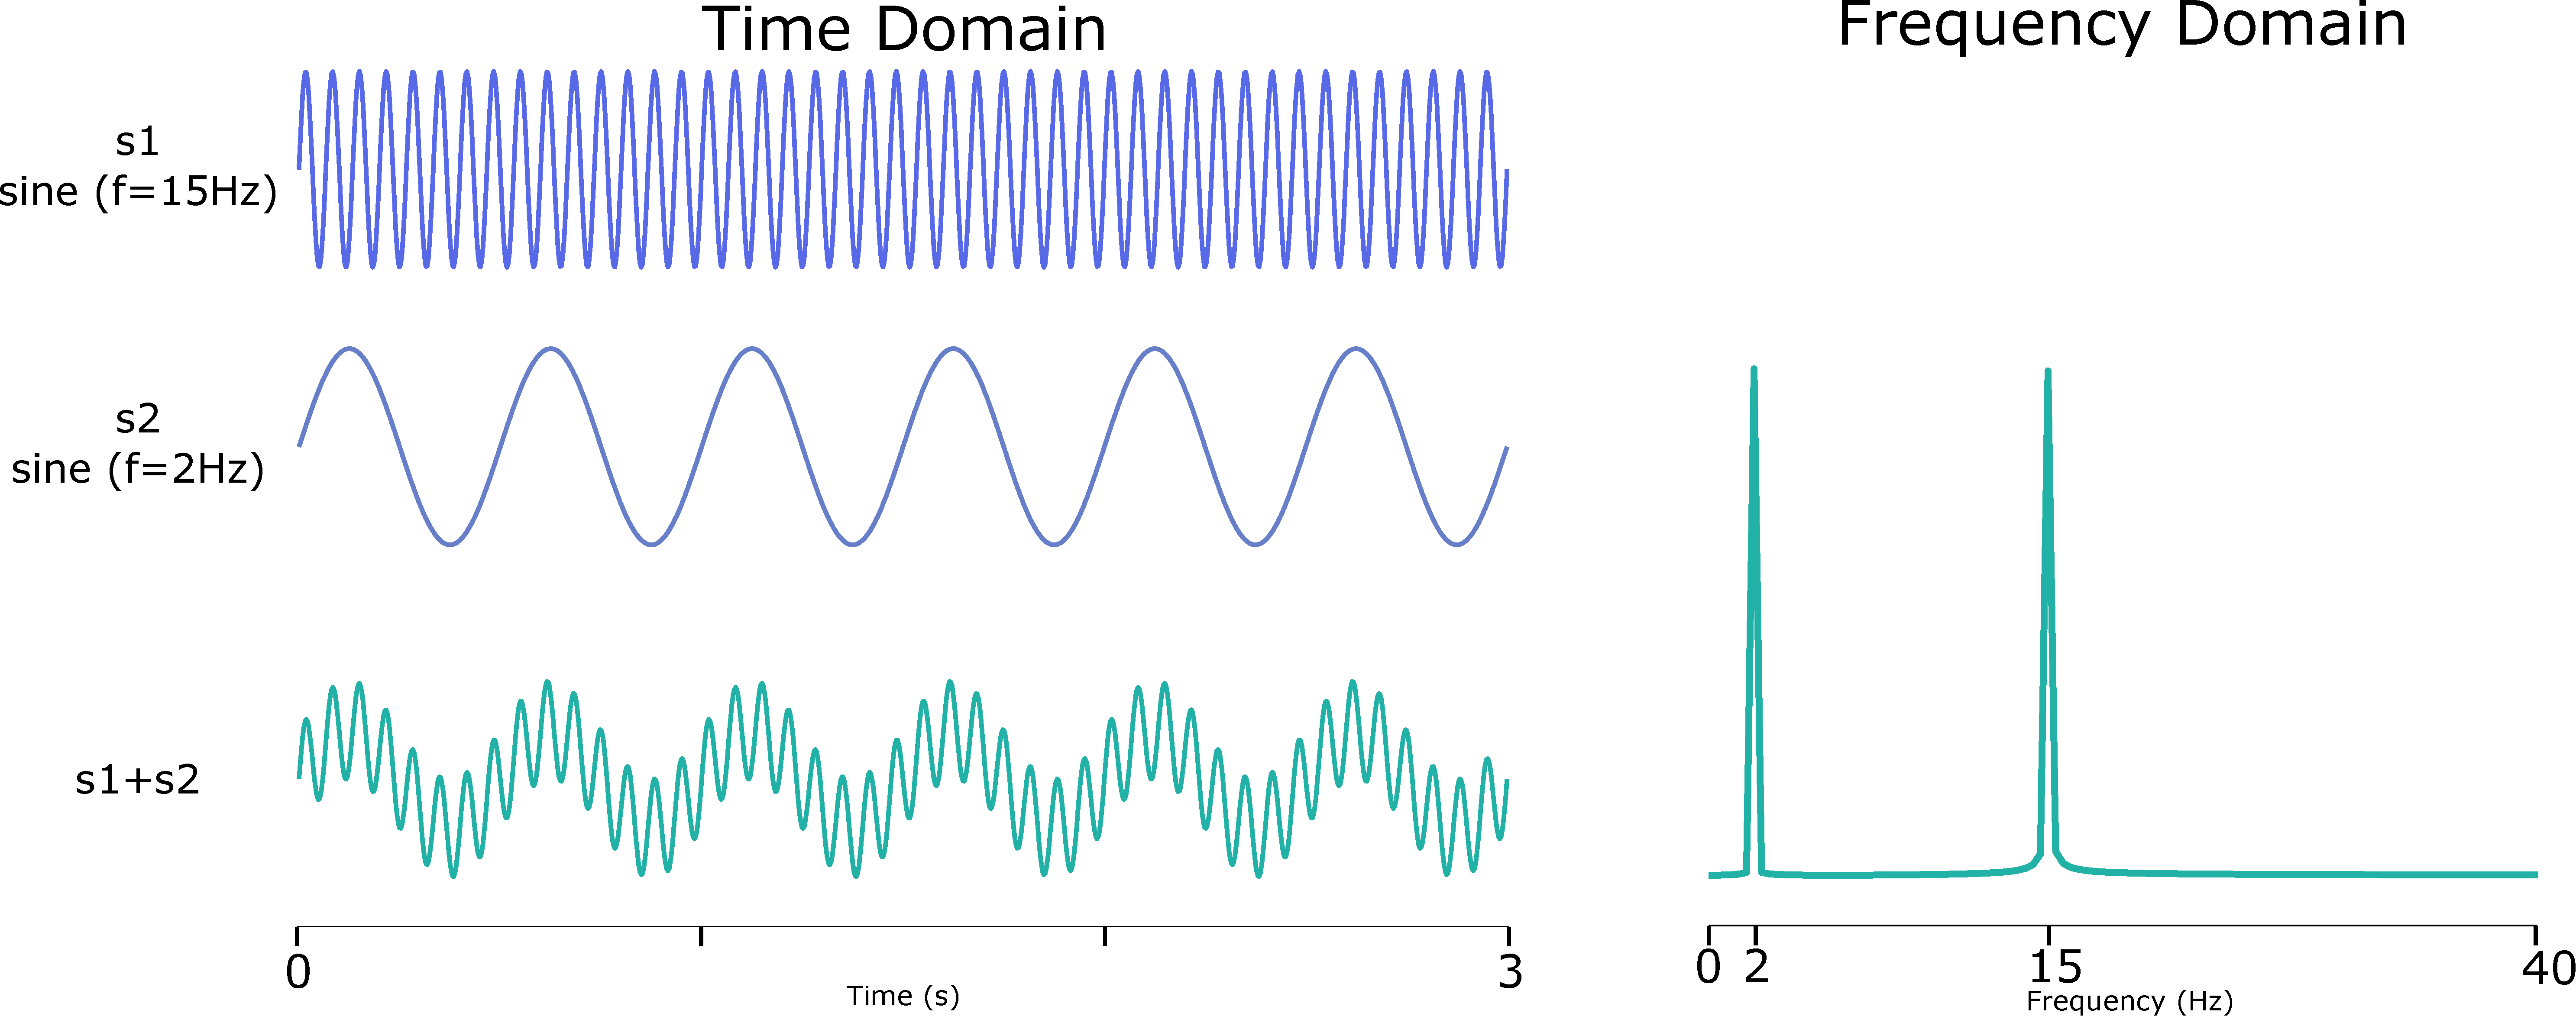
\includegraphics[width=\linewidth]{fourier.pdf}
    \caption{\gls{dft} of a sum of sine waves.}
    \label{fig:fourier}
\end{figure}

One of the first and most well-known techniques suggested for time series transformation is the \gls{dft} \cite{fourier}. The idea behind this concept is that any signal, either periodic or not, is a decomposition of a finite number of sine and cosine waves, from which amplitude and phase are used to represent the signal in the frequency domain \cite{fourier2}. This transformation allows us to see the signal differently, highlighting which frequencies concentrate more or less energy. It unveils the presence of specific types of noise or artifacts, or periodic shapes. Figure \ref{fig:fourier} shows the transformation of a signal into the frequency domain. The signal is the sum of two different sine waves with 2 and 15 Hz respectively. The result of the Fourier transform is a frequency series with high energy at the frequencies of the sine waves.

The frequency domain opens new possibilities for the analysis of the time series, namely for the extraction of spectral features, which are also used to represent the signal in the feature domain. 

\subsection{Feature-based Representation}
\label{subsec:features}

\begin{figure}[!h]
\centering
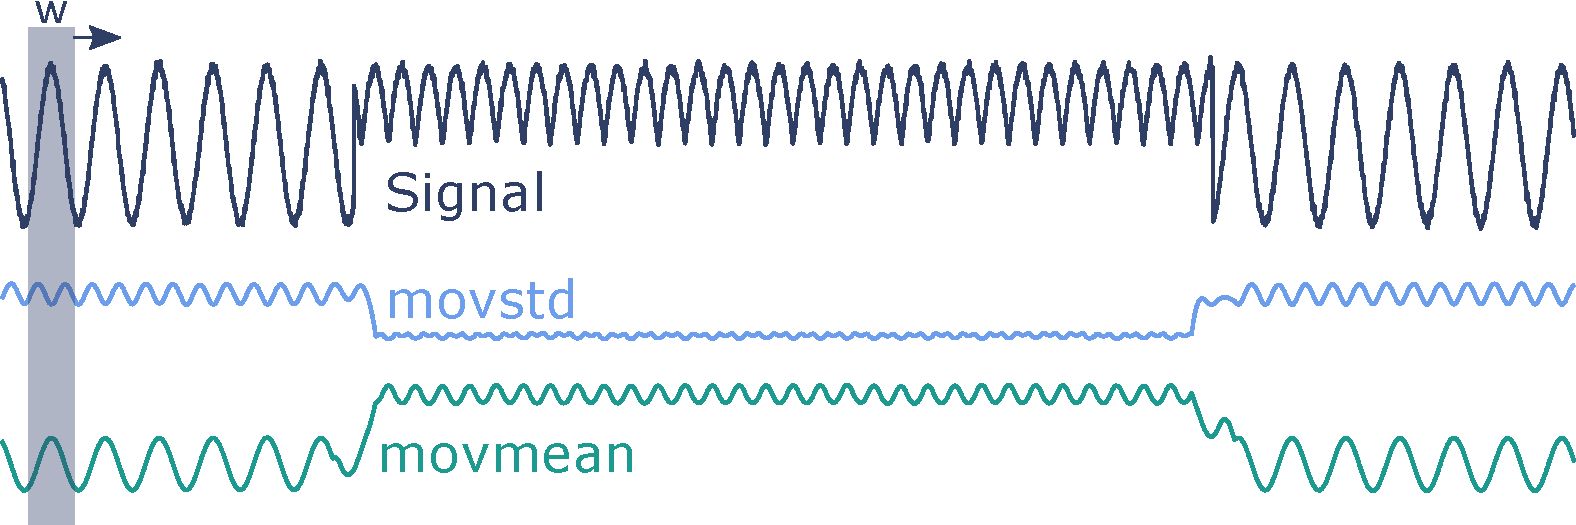
\includegraphics[width=\linewidth]{features.pdf}
\caption{Moving window used to extract features with total overlap. The mean and standard deviation are extracted from the signal. The left shows the sine waves, while the right shows the frequency spectrum of the combination of sine waves.}
\label{fig:feature_intro}
\end{figure}

The process of feature extraction is also a transformation method commonly employed and is performed by a \textit{moving window}, resulting, for each feature, in a feature series (see Section \ref{sec:global}). In Figure \ref{fig:feature_intro} is shown a time series from which the average (moving mean) and standard deviation (moving \textit{std}) are computed with a moving widow of size $w=100$ and a total overlap $o=100\%$. The feature is a characterization of the signal for that specific extracted property and is commonly used in machine learning tasks. In this thesis we will present two main applications of the feature representation of time series.

\subsection{Piecewise Aggregate Approximation}
\label{subsec:paa}

\begin{figure}[!h]
\centering
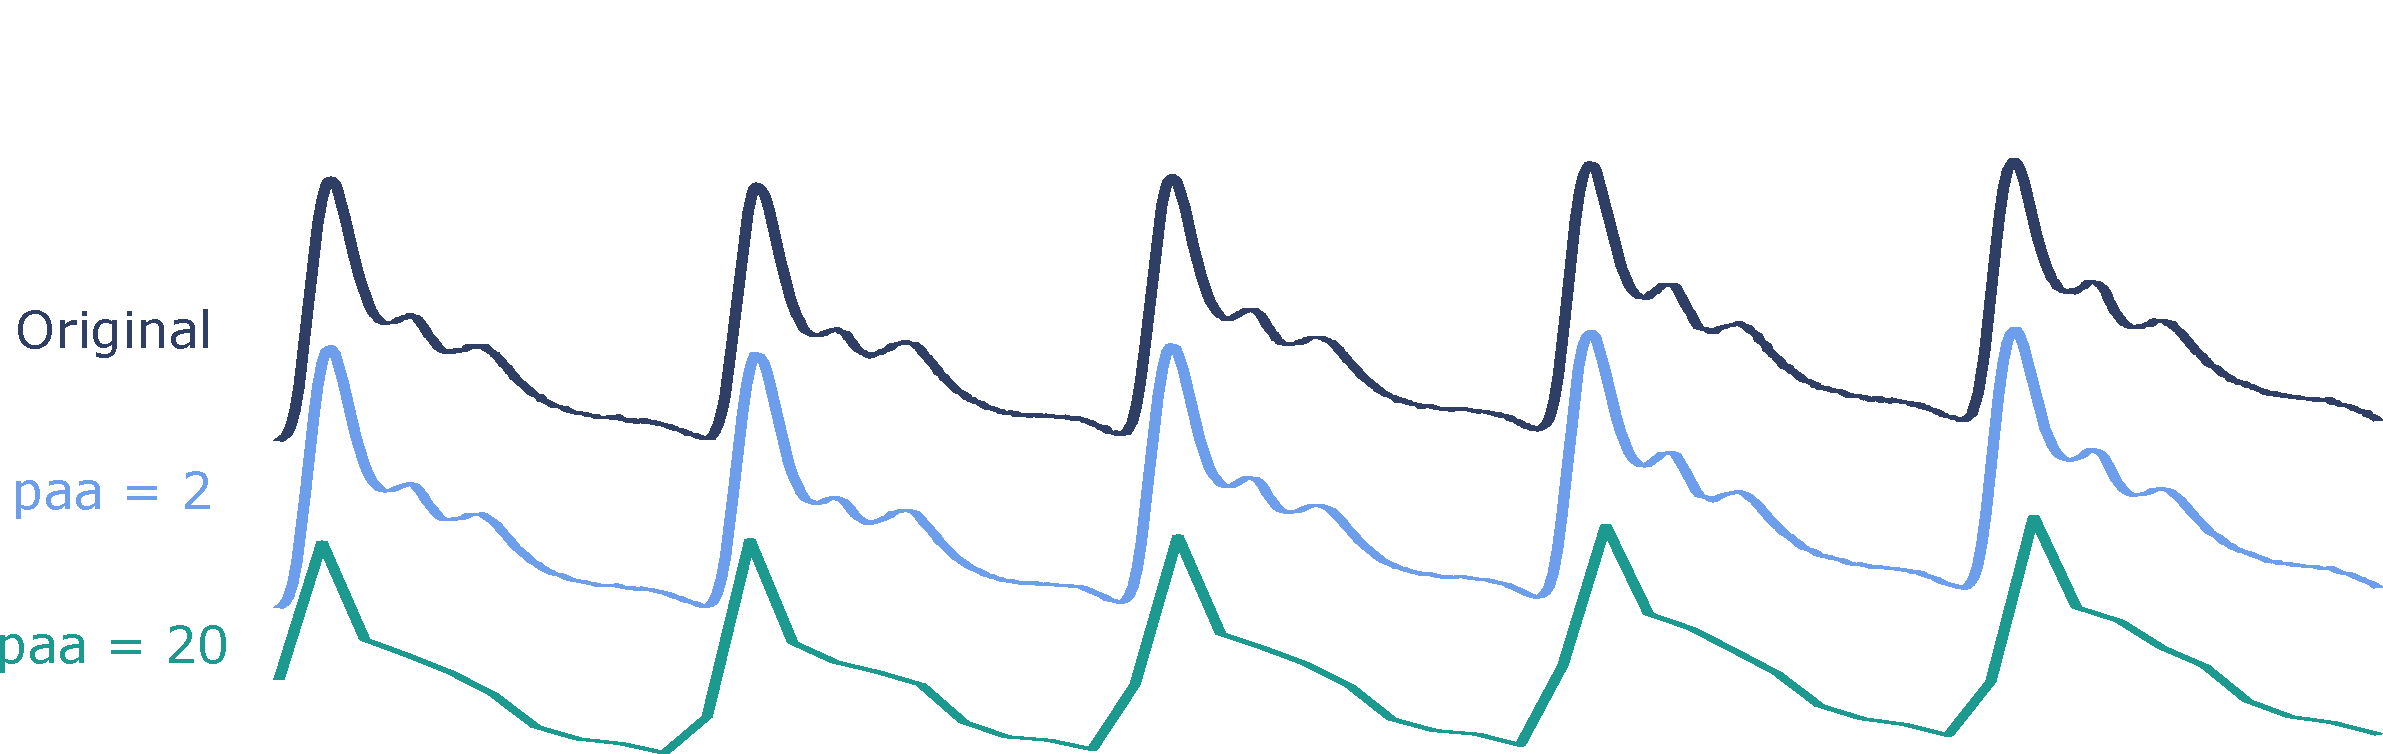
\includegraphics[width=\linewidth]{paa_bvp.pdf}
\caption{\gls{paa} representation of a \gls{abp} signal, with window sizes of 2 and 20, repsectively. The \gls{paa} representation was computed with the \gls{pyts} module \cite{pyts}, based on \cite{paa}.}
\label{fig:paa}
\end{figure}

Another common used transformation method to simplify a time series and reduce its dimension is the \gls{paa}) \cite{paa}. The new representation space will have size $1 < N \leq n$, in which $N$ is a factor of the original size $n$. The method searches to keep the average of the \textit{N} equi-sized \textit{subsequences} in which the original signal with length \textit{n} is segmented, which results in $\overline{T} = \overline{t_1}, \overline{t_2}, ...,\overline{t_N}$, such that \cite{paa}:

\begin{equation}
\overline{t_i} = \frac{N}{n} \sum^{\frac{n}{N}i}_{j=\frac{n}{N}(i-1)+1} t_j.
\end{equation}

An example is shown in Figure \ref{fig:paa}, where a \gls{abp} signal is transformed into a \gls{paa} with sizes 2 and 20, respectively.
    
\subsection{Symbolic Aggregate Approximation}
\label{subsec:sax}

\begin{figure}
\centering
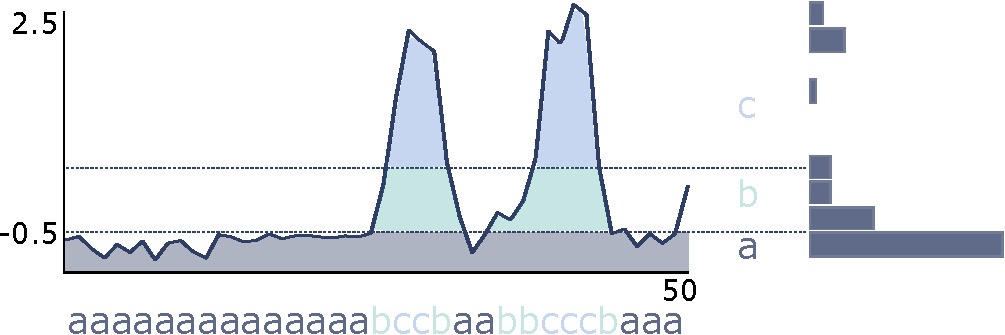
\includegraphics[width=\linewidth]{sax_test.pdf}
\caption{\gls{sax} representation of a power consumption signal from a Dutch Company, with window bin size of 3. The \gls{sax} representation was computed with \gls{pyts} based on \cite{sax}.}
\label{fig:sax}
\end{figure}

From this method, a new representation technique was born, transforming the signal from the numerical to the symbolic domain. It is called \gls{sax} \cite{sax}. This method applies \gls{paa} to a z-normalized time series and indexes a \textit{character} to each sample of the simplified signal based on the distribution of its amplitude values \cite{sax}. The signal's amplitude values are separated in bins with equal probability. The number of bins is equal to the size of the symbolic \textit{alphabet} chosen. Figure \ref{fig:sax} shows an example of the signal transformed into a string with 3 letters in its alphabet. Such as the \gls{dft}, \gls{sax} brings novel ways of analising time series in a completely different manner, profiting from the much-acquired knowledge in text mining.

This representation method is relevant to be introduced as it was a strong inspiration for the proposed novel symbolic representation technique for time series. Ultimately used for expressive pattern search and classification. 

In order to perform pattern search or classification tasks, we have to calculate the difference/similarity between two time series or \textit{subsequences}.

\section{Distance Measures}
\label{sec:distance}

There is a large number of distance measures for time series, but two of the classical and standard measures still provide state-of-the-art results in most time series data mining tasks, namely the \gls{ed} and the \gls{dtw}.

\subsection{Euclidean Distance}
\label{subsec:ed}

The \gls{ed} is the most straightforward distance measure for time series. Let us consider two time series, $Q$ and $C$, of length $n$, so that\\
\\
$Q = q_1, q_2, ..., q_i, ..., q_n$\\
$C = c_1, c_2, ..., c_i, ..., c_n$\\

The distance between these two time series under the \gls{ed} is:

\begin{equation}
ED(Q,C) = \sqrt{\Sigma^n_{i=1} (q_i - c_i)^2},
\end{equation}

which represents the square root of the sum of the squared amplitude differences between the samples of each signal. Although the distance measure is simple to compute, it is highly susceptible to typical distortions on time series. When using \gls{ed}, these distortions must be removed, otherwise, other methods, invariant to these distortions, should be used. Examples of distortions are amplitude and offset distortion, phase distortion, and local scaling ("warping") distortion. The first can be compensated by the z-normalized \gls{ed} \cite{complexity}:

\begin{equation}
\label{eq:norm_ed}
z\_ED(Q,C) = \sqrt{2m(1-\frac{\Sigma^m_{i=1}Q_iC_i - m\mu_Q\mu_C}{m\sigma_Q\sigma_C})},
\end{equation}

where $\mu_Q$ and $\mu_C$ are the mean of the time series pair and $\sigma_Q$ and $\sigma_C$ are the standard deviation.

The \textit{warping} distortion can be solved with an elastic measure. For this purpose, \gls{dtw} is typically used.

\subsection{Dynamic Time Warping}
\label{subsec:dtw}

\begin{figure}
\centering
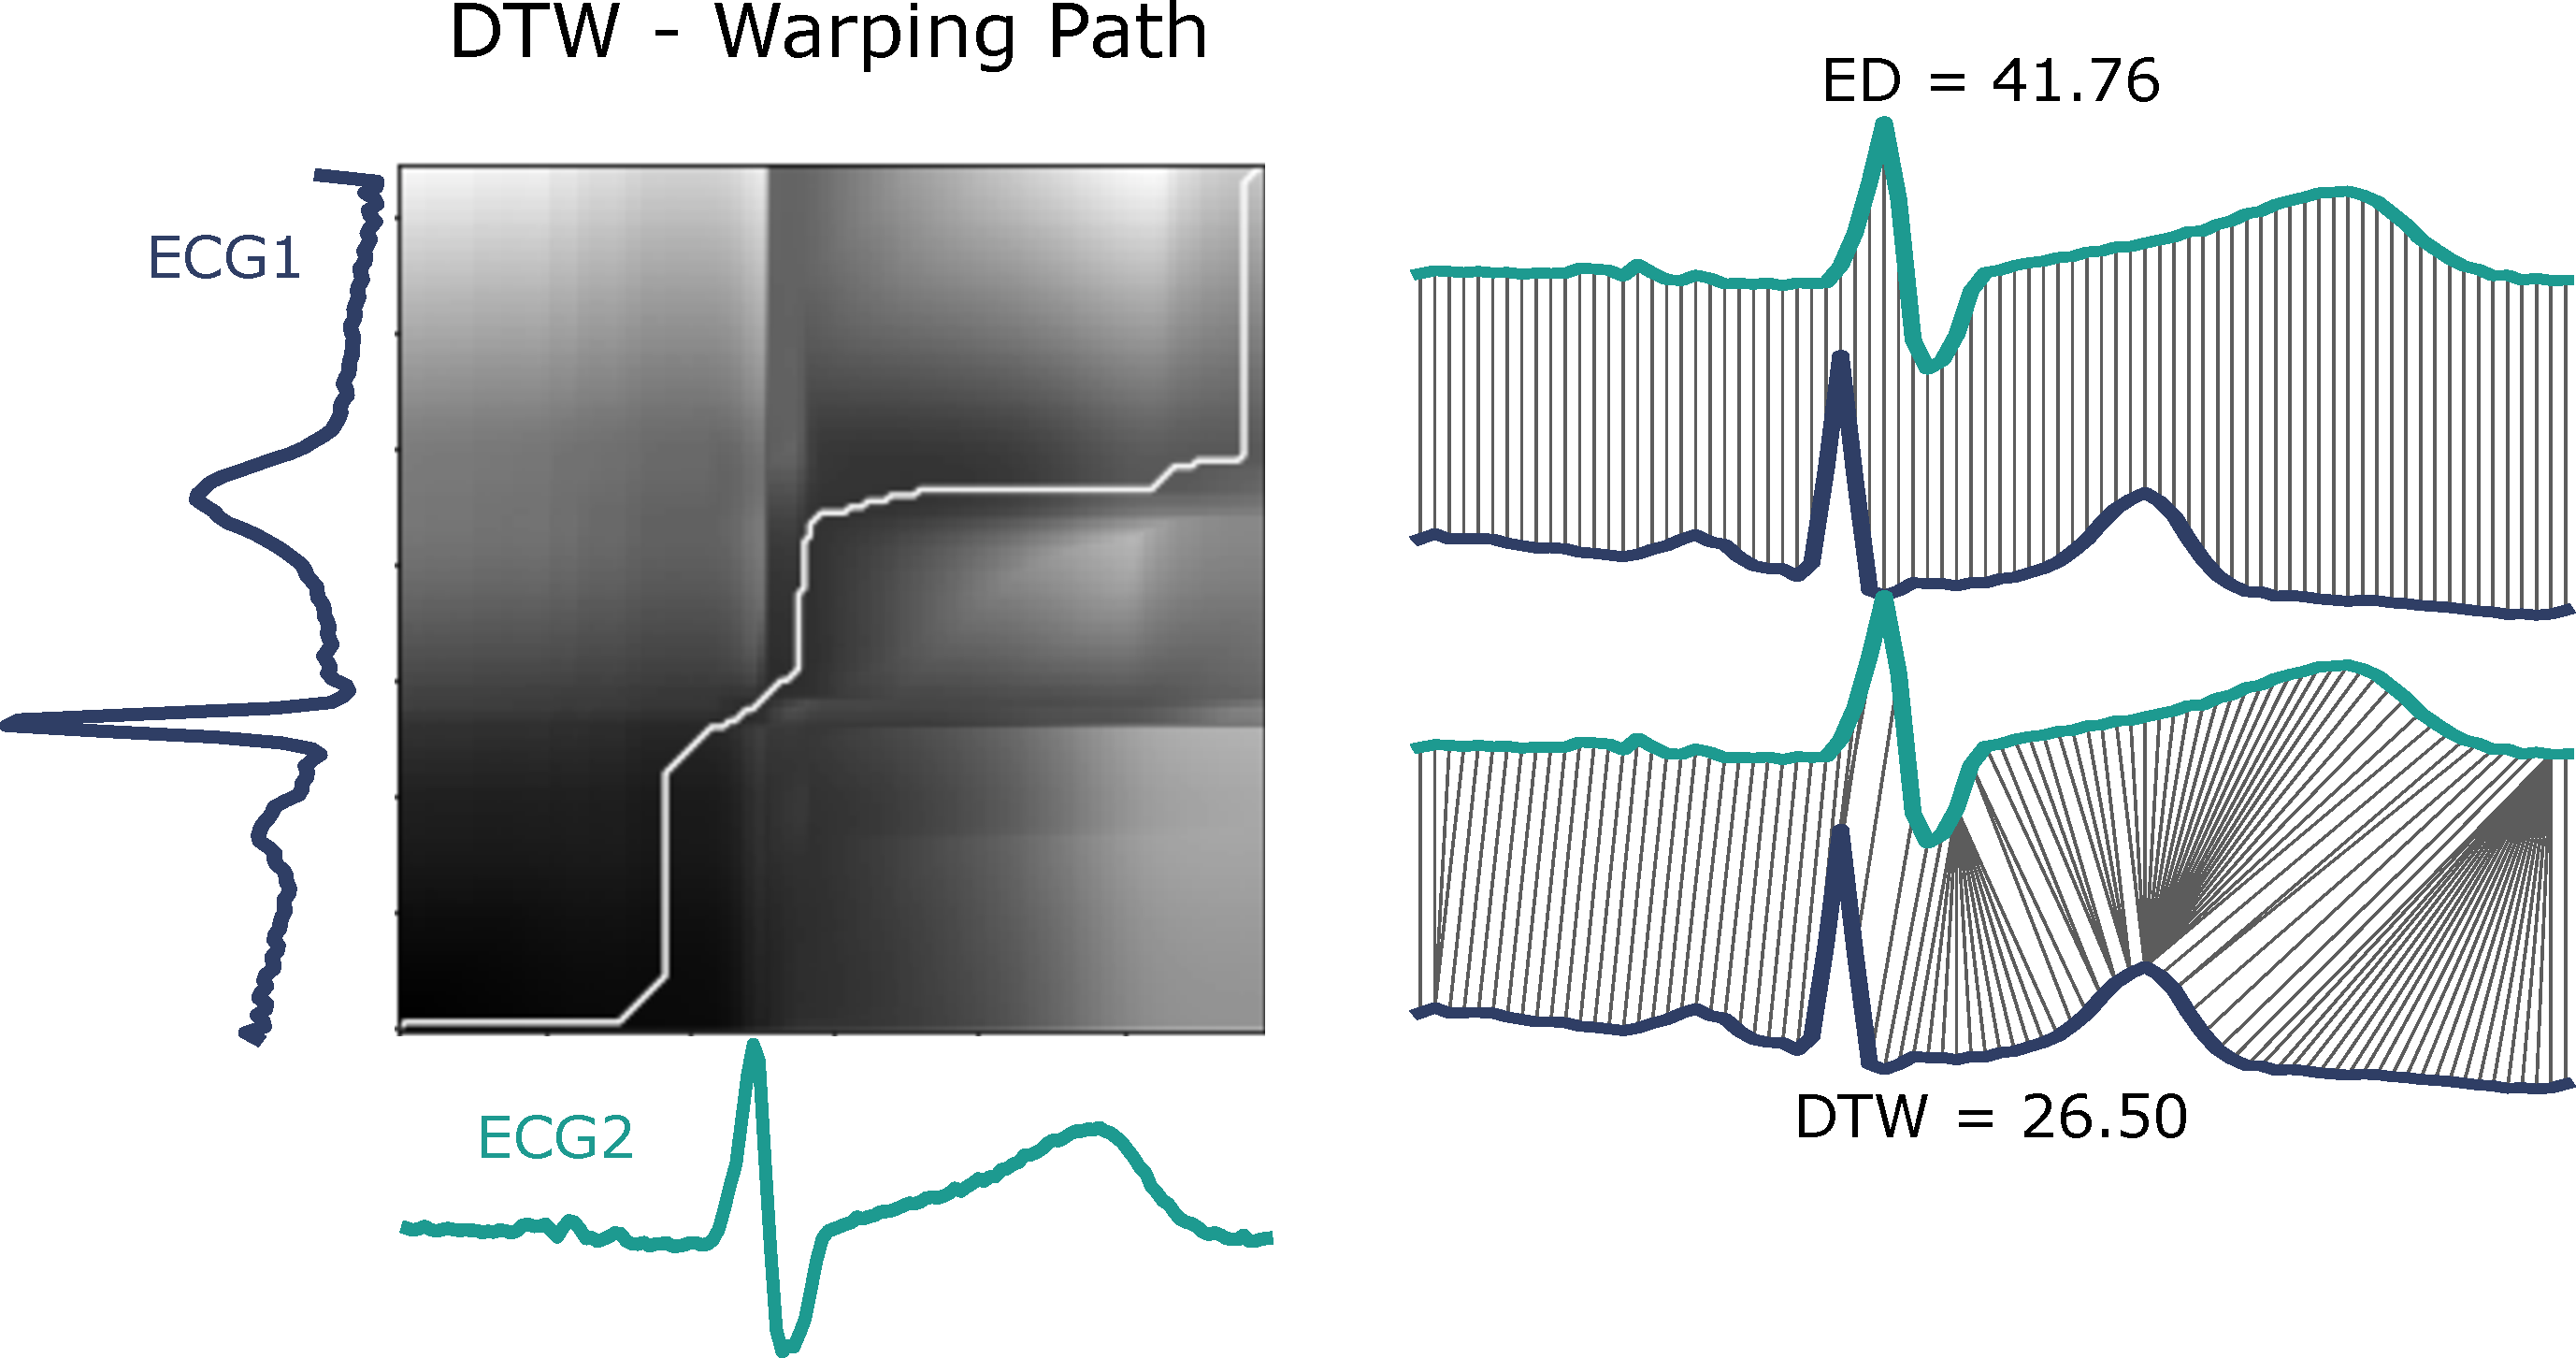
\includegraphics[width=\linewidth]{dtw.pdf}
\caption{\gls{dtw} and \gls{ed} distances on two different \gls{ecg} signals.}
\label{fig:dtw_intro}
\end{figure}

The \gls{dtw} distance measures the alignment between two time series. Let us consider two time series, $Q$ and $C$, of length $n$ and $m$, respectively:\\
\\
$Q = q_1, q_2, ..., q_i, ..., q_n$\\
$C = c_1, c_2, ..., c_j, ..., c_m$\\
\\
The alignment is measured by means of a distance matrix with size $n$-by-$m$, where the $(i^{th},j^{th})$ cell of the matrix contains the $d(q_i, c_j)$ between the two points $q_i$ and $c_j$, being $d=(q_i - c_j)^2$ \cite{dtw}. Figure \ref{fig:dtw_intro} shows an example of a distance matrix between two time series. The matrix fully describes the difference between the two time series and maps where these align. The mapping is made by a warping path, $W$, that represents the set of matrix cells that minimize the warping cost, also defined as the cumulative distance of these cells \cite{dtw}.

\begin{equation}
W = w_1, w_2, ..., w_k, ..., w_K; \quad \quad max(m,n) \leq K < m+n+1,
\end{equation} 

\begin{equation}
DTW(Q,C) = min \sqrt{\Sigma^K_{k=1} w_k}.
\end{equation} 

The cumulative distance $\gamma(i,j)$ is calculated as $d(q_i,c_j)$ of the current cell added to the minimum distance adjacent to that cell:

\begin{equation}
\gamma(i,j) = d(q_i,c_j)+min\{\gamma(i-1,j-1), \gamma(i-1, j), \gamma(i, j-1)\}.
\end{equation} 

When two time series with the same length have a linear warping path, such that $w_k=(i,j)_k, i=j=k$, we have a special case of the \gls{ed}. \gls{dtw} has a time and space complexity of $O(nm)$ while the \gls{ed} has linear complexity ($O(n)$). Figure \ref{fig:dtw_intro} shows an example of applying the \gls{ed} and \gls{dtw} on two different \textit{PQRS} complexes from different \gls{ecg}s. 

\subsection{Complexity Invariant Distance}
\label{subsec:complexity}

A different type of distance measure is also used to cope with complexity invariances. This distance uses a complexity correction factor ($CF$) with an existing distance measure, such as \gls{ed} \cite{complexity}:

\begin{equation}
CD(Q,C) = ED(Q,C)\times CF(Q,C).
\end{equation}

The $CF$ is defined as \cite{complexity}:

\begin{equation}
CF = \frac{max\{CE(Q),CE(C)\}}{min\{CE(Q),CE(C)\}},
\end{equation}

where $CE$ represents the complexity estimate of a time series. This estimate is calculated based on the intuition that if we could  "stretch" a time series until it becomes a straight line, this line would be as long as the complexity of the signal. It can be computed as the sum of the $n-th$ discrete differences along the time series \cite{complexity}:

\begin{equation}
\label{eq:complexity}
CE(Q) = \sqrt{\Sigma^{n-1}_{i=1} (q_i - q_{i+1})^2}.
\end{equation}

These distance measures are performed on the original representation domain of the time series. As we showed above, other representation techniques can be employed, creating opportunities for other types of approaches. In this work, we propose other representation techniques to create novel ways of exploring time series. Therefore, other distance measures that can be used in different representations of time series will be explained. 

\subsection{Feature-based Distance}
\label{subsec:features_dist}

As mentioned, a feature series $F$ can be computed from the original time series to represent it based on a specific feature.  Each \textit{subsequence} scanned by the \textit{moving window} is characterized by the feature value, and a $F$ is computed as an array. When multiple features are extracted, each \textit{subsequence} is characterized by a set of features, creating a feature vector $\vec{f}$ with $r$ feature values (to be clear, a feature vector is the set of feature values for a \textit{subsequence} of the time series, while a feature series is a feature representation of the entire time series). 
\par
Vector-based distance measures can be used with feature vectors to compare different time series or \textit{subsequences}. There are several vector-based distance measures, including the already mentioned \gls{ed} or the manhattan distance, but we will only describe the cosine similarity/distance.
\par
The cosine similarity is a measure of the angle between two vectors determining if these are pointing in the same direction. Consider two feature vectors $\vec{f_A}$ and $\vec{f_B}$. Their cosine similarity is computed as their normalized dot product \cite{cosine} (equation \ref{eq:cosine}).

\begin{equation}
\label{eq:cosine}
CS = \frac{\vec{f_A} \cdot \vec{f_B}}{||\vec{f_A}|| ||\vec{f_B}||}
\end{equation}

being $||\vec{f_A}||$ and $||\vec{f_B}||$ the euclidean norm of each feature vector, defined as $\sqrt{\Sigma_{i=1}^{r} f_{Ai}^2}$ and $\sqrt{\Sigma_{i=1}^{r} f_{Bi}^2}$, respectively \cite{cosine}. Because the cosine similarity includes a vector normalization, it does not rely on the magnitude of the vectors and the difference is solely due to the angle between vectors. This is relevant for domains where vectors have high dimensionality, which is the case for feature vectors.


\section{Applying Distance Measures}
\label{sec:dist_measures}

Measuring distances between time series allows to compare them. It is the fundamental instrument for most time series data mining tasks. With a distance measure, we can compare groups of time series for classification purposes or compare \textit{subsequences} with a query template to find if it occurs in the time series. Not only can we compare different time series, but also compare the time series with subsequences of itself. By comparing each of its \textit{subsequences} to all other \textit{subsequences}, relevant structural information becomes available. In this subsection, relevant methods applied with the help of the presented distance measures are explained to retrieve information from a time series. We will start with distance/similarity profiles.

\subsection{Distance Profile}
\label{subsec:matrixprofile}

As mentioned in the previous subsection, measuring all the distance pairs of a time series provides the ability to retrieve relevant structural information. When computing the distance of a \textit{subsequence} to all the other \textit{subsequences} of the time series, a \textit{distance profile} is calculated. Each \textit{subsequence} can have a \textit{distance profile} and when computing all the distance pairs, a self-distance matrix is the result.
\par
Recently, a strategy was proposed to compute a one-dimensional distance \textit{profile} for a time series based on a z-normalized \gls{ed} matrix. By keeping the lowest value of each \textit{distance profile} (nearest \textit{subsequence}), we retrieve the \textit{matrix profile} \cite{eamonn1}. The result gives the minimal distance pair of each \textit{subsequence}, meaning that minimum values are \textit{motifs} and maximum values are \textit{discords}.\\\\
\textbf{Motif:} The \textit{subsequence} pair that has the lowest distance forms a motif. That means that on the entire time series, these two \textit{subsequences} are the closest ones. The opposite is a \textit{discord}.\\\\
\textbf{Discord:} The \textit{subsequence} pair that has the highest distance forms a \textit{discord}. That means that on the entire time series, these two \textit{subsequences} are the furthest apart.\\

\subsection{Self-Distance Matrices}
\label{subsec:dist_matrix}

\begin{figure}
\centering
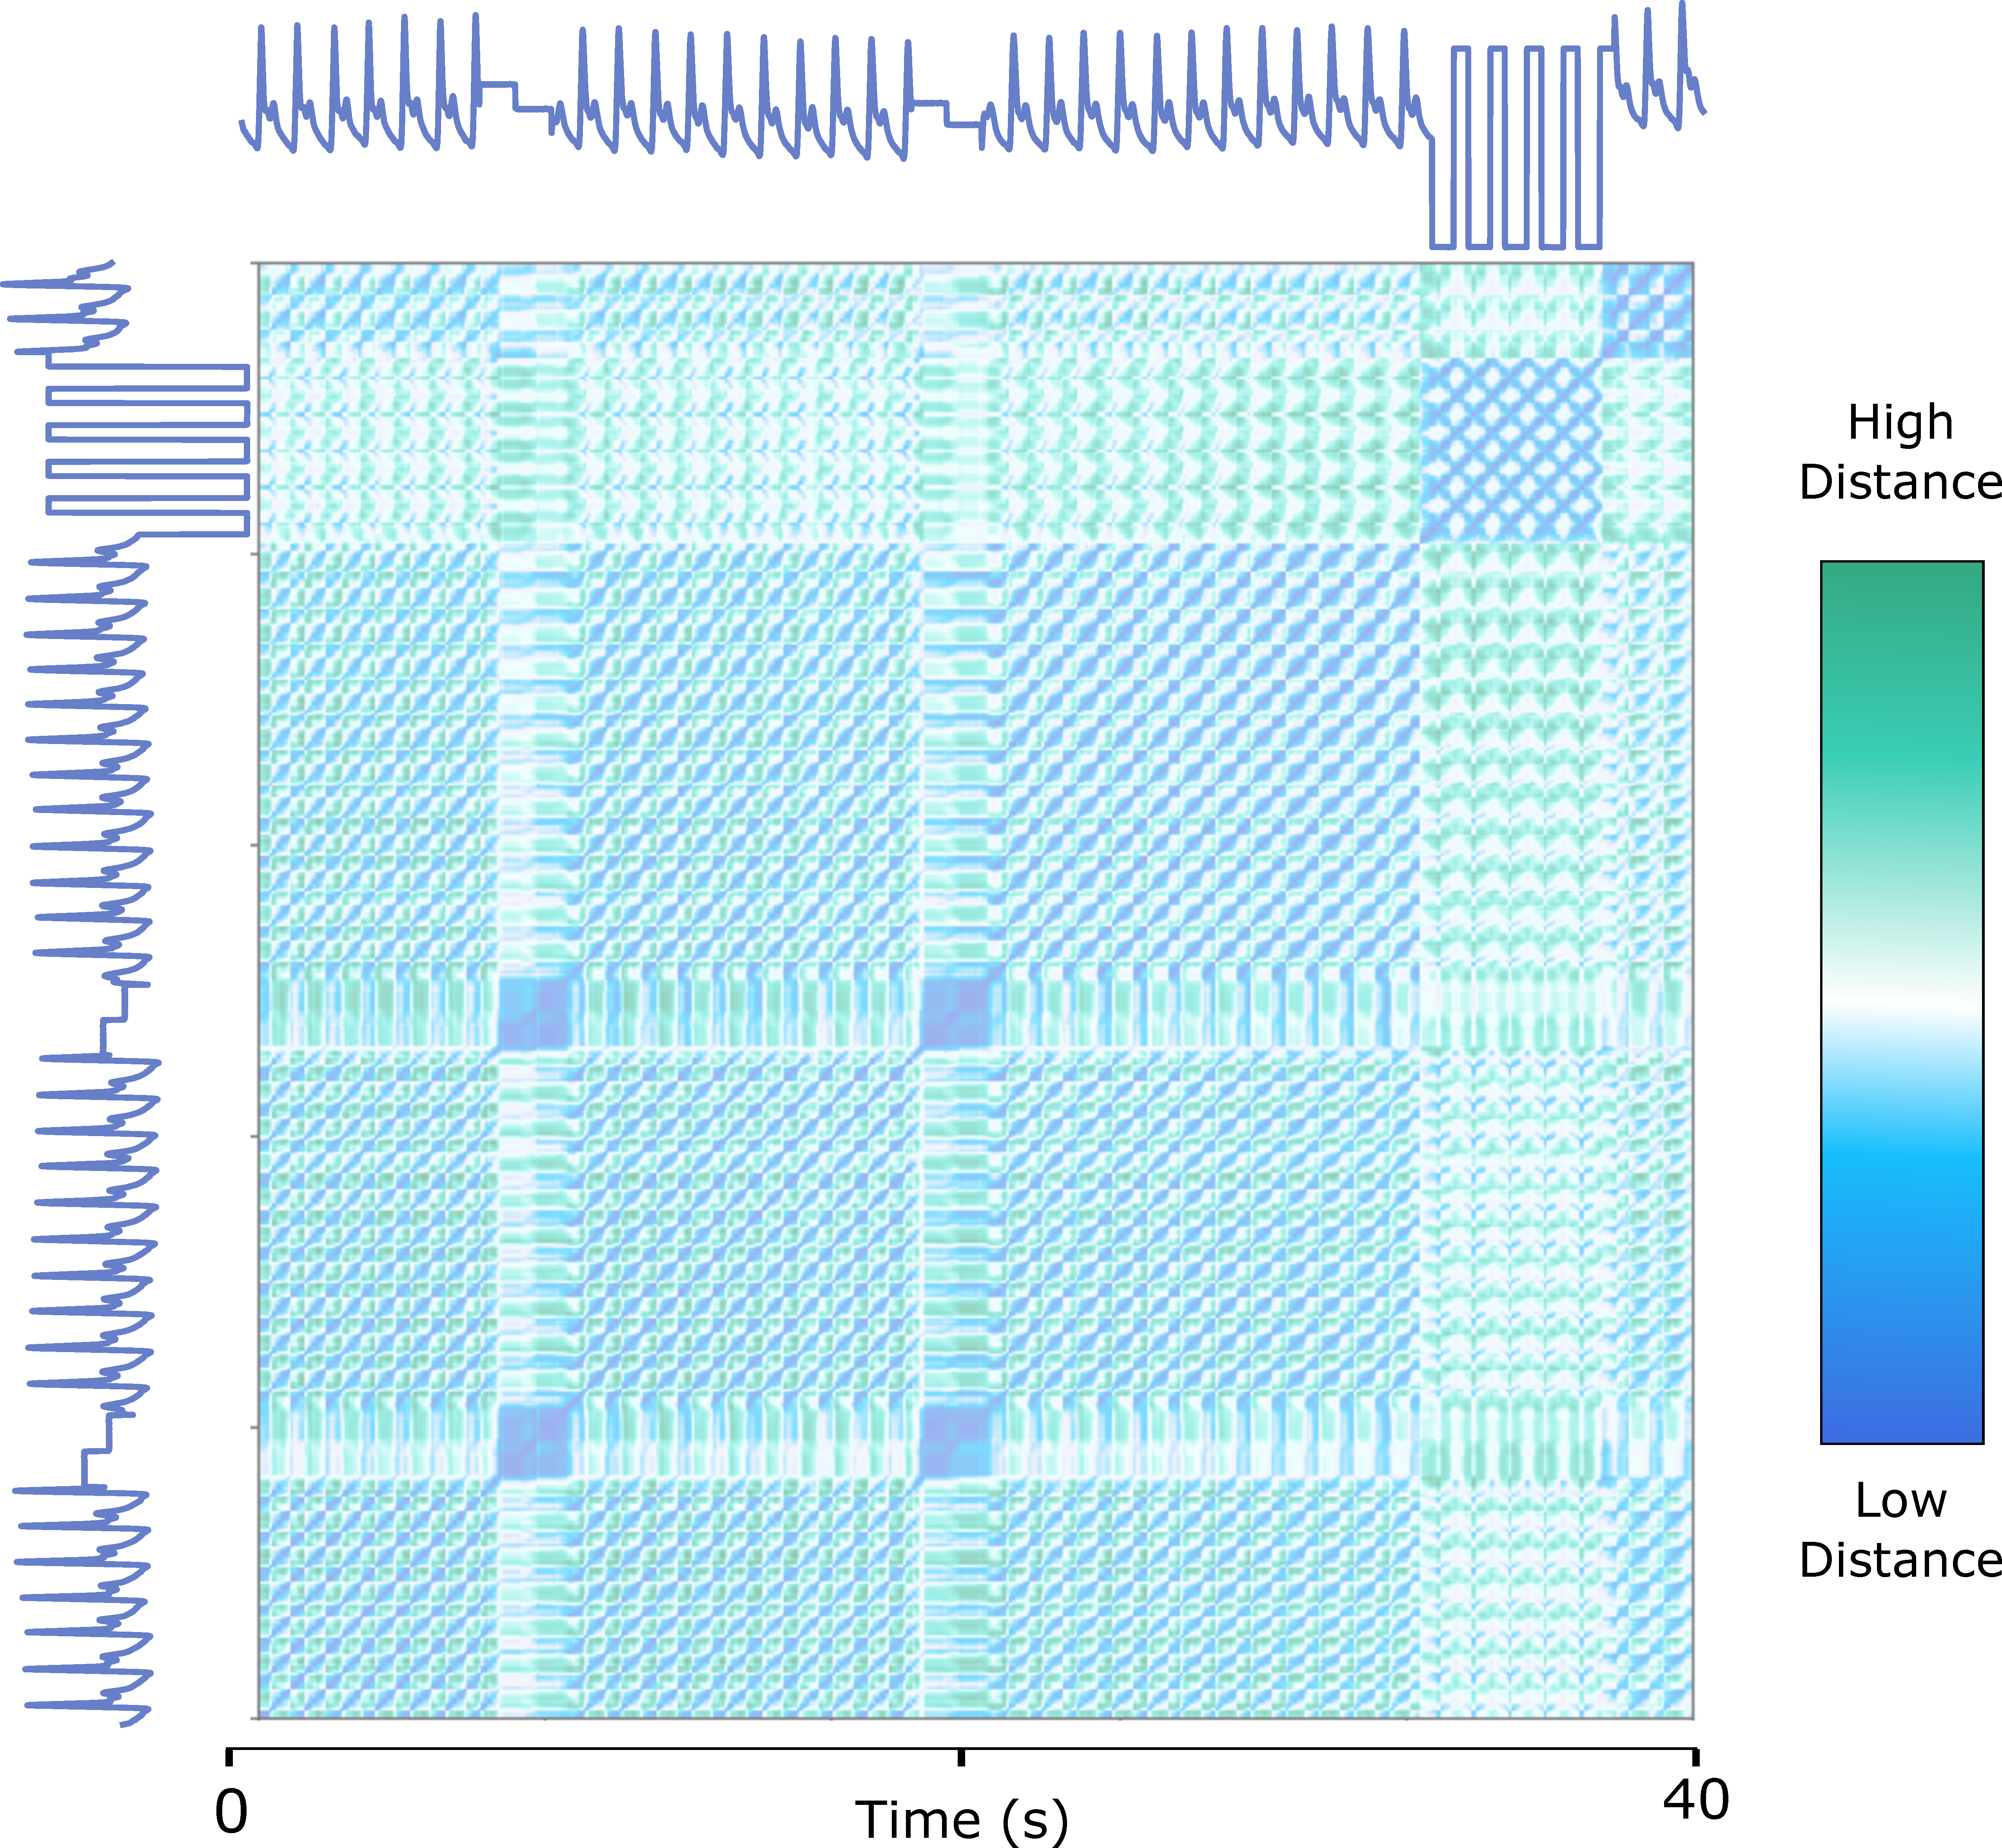
\includegraphics[width=0.85\linewidth]{Chap2Sec362.pdf}
\caption{Self-Distance Matrix (SDM) representation of the \gls{abp} signal. The matrix was computed using the cosine distance between the feature representation of the signal. The main structures that can be highlighted are \textit{blocks} along the main diagonal of the matrix, \textit{paths} that are parallel to the main diagonal, and \textit{cross-paths} that are perpendicular to the main diagonal. The signal comes from a public dataset (see Section \ref{dat:dataset2}).}
\label{fig:ssm_pre}
\end{figure}

A time series can reveal relevant information when each \textit{subsequence} is compared to all the other \textit{subsequences} of the same time series. The result is a pairwise distance matrix that unveils \textit{homogeneity}, \textit{repetition} and \textit{novelty} on the time series \cite{fmp1}. Each are relevant for segmentation and summarization tasks.

Let $X$ be a sequence with size $N \in \mathbb{N}$ that can be a time series or a representation of a time series in the \gls{paa} or feature space, such that $X = (x_1, x_2, ..., x_i, ..., x_j, ..., x_N)$. Each element of $X$ can either be a single value or a vector with $r$ features. Independently of that, a matrix $SDM$ with size $N \times N$ can be computed, such that:

\begin{equation}
\label{eq:sdm}
SDM(i,j)= d(x_i, x_j),
\end{equation}

being $d$ a distance measure between elements $x_i, x_j \in X$ for $i, j \in [1:N]$. $SDM(i,j)$ represents a cell of $SDM$ that contains the distance value. When $i=j$ the distance should be zero, therefore the diagonal of $SDM$ has the lower values. Besides the main diagonal, other relevant structures can be found in $SDM$. These include \textit{homogeneous blocks} and \textit{paths} \cite{fmp1, fmp2}, as can be seen in Figure \ref{fig:ssm_pre}.

Areas with lower distance and block structure along the diagonal are highlighted as \textit{homogeneous} segments. These give an indication of \textit{homogeneity} and \textit{novelty}. \textit{Homogeneity} because a \textit{block} along the diagonal means that the time series has a constant behaviour during the segment delimited by the \textit{block}. \textit{Novelty} because when $SDM$ has multiple \textit{blocks} along the diagonal, it shows that the time series shifted its behaviour/regime. The moment there is a transition between \textit{blocks} is a potential segmentation point. In Figure \ref{fig:ssm_pre}, changes in the \gls{abp} signal are visible as blocks. In total, seven regimes are present on the signal, and seven blocks can be counted along the main diagonal.

\begin{figure}
\centering
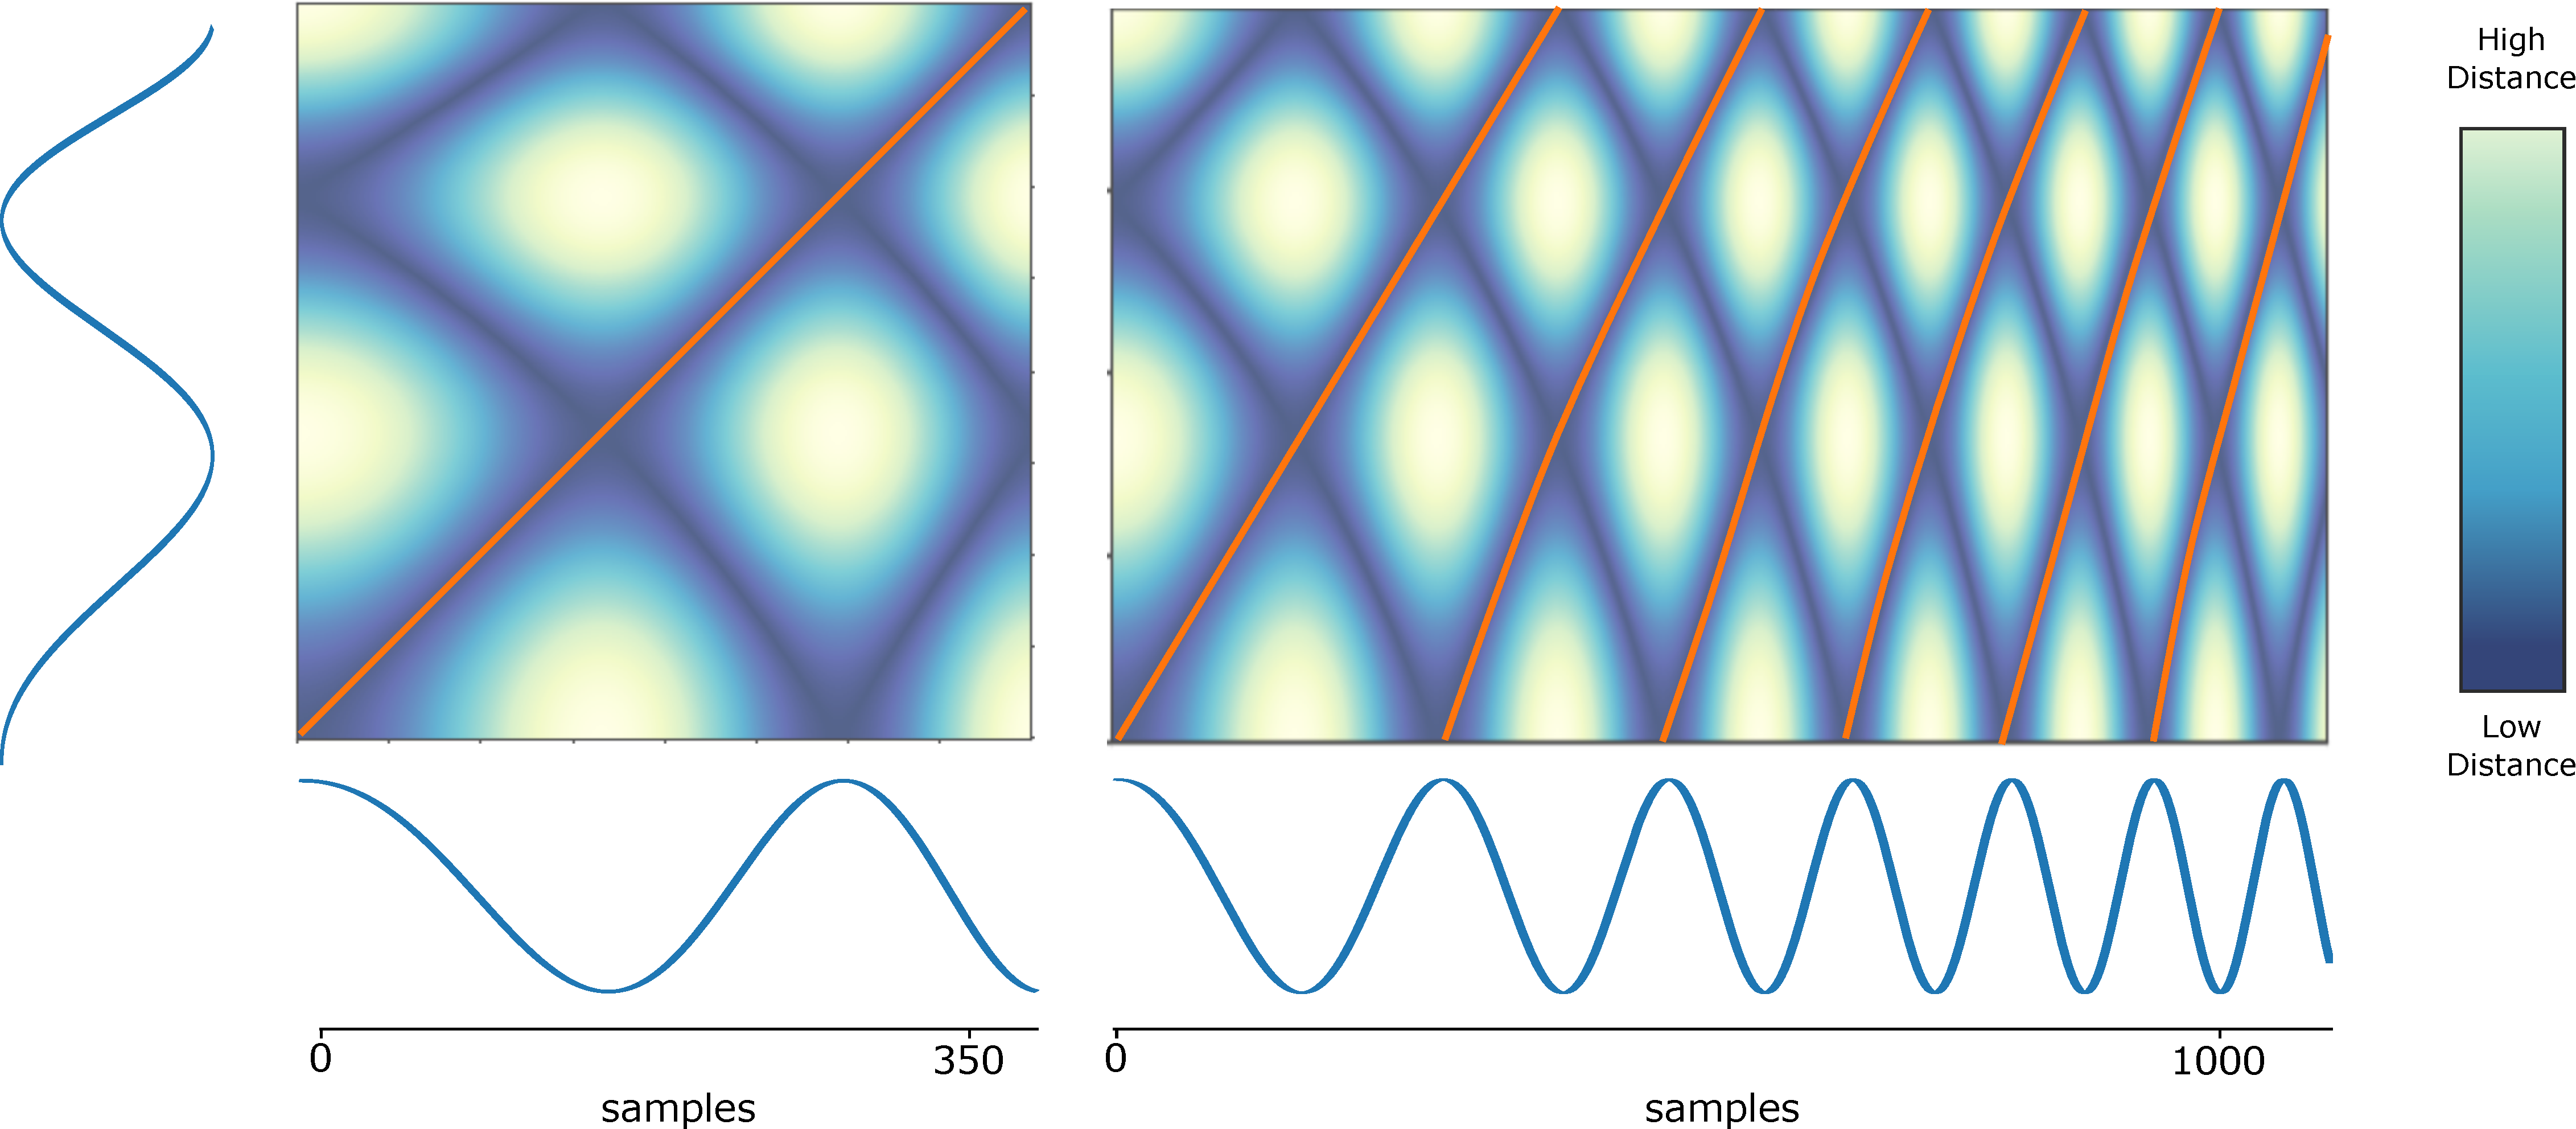
\includegraphics[width=\linewidth]{Chap2Sec362_Paths.pdf}
\caption{$SDM$ of a chirp signal computed with the pairwise euclidean distance. The chirp signal is a sine wave with increasing frequency (in this case from $f_0$=1Hz and $f_1$=25Hz)\cite{scipy}. Left) \textit{Subsequence} of the chirp signal compared with itself. Right) The same \textit{subsequence} is compared with the entire chirp signal.}
\label{fig:sdm_periods}
\end{figure}

Repeating \textit{subsequences} in the time series are represented by \textit{paths} on $SDM$. \textit{Paths} are observed on the $SDM$ because of matching \textit{subsequences} during the sliding process, which computes consecutive low distance values represented in a diagonal form on the matrix. If the \textit{subsequences} being compared are exactly the same, the diagonal is perfect, but differences might be found, which results in a distorted diagonal. In Figure \ref{fig:sdm_periods} we show an example of an $SDM$ with a chirp signal that has a continuously increasing frequency. A \textit{subsequence} of the signal is compared with itself (Figure \ref{fig:sdm_periods}.left) and with the entire chirp signal (Figure \ref{fig:sdm_periods}.right). We highlighted the relevant \textit{paths} in orange. When comparing the signal with itself only, the \textit{path} is a perfect straight line, but when compared with the entire signal, the \textit{paths} are continuously more distorted and shorter. These show where each period of the sine wave occurs, and the distortion results from the increasing frequency of the signal. In the $SDM$ from Figure \ref{fig:ssm_pre}, \textit{paths} are visible on the matrix, indicating the presence of periodicity. The \textit{cross-paths} indicate the same periodic behaviour, but also that the \textit{subsequence} is symmetric.

It is relevant to highlight that as distance matrices can be computed, similarity matrices can as well, by following the same equation \ref{eq:sdm}, but using a similarity measure ($s$) instead of $d$. Further in this manuscript, we will only mention the similarity matrix, which will be called \gls{ssm}, as the proposed method uses the cosine similarity.

\subsection{Template-based Search}
\label{subsec:query_based_search}

The presented distances can also be used to retrieve a distance profile from a \textit{template}. This type of mechanism belongs to the class of query-based search problems. The process to compute this distance profile involves sliding the template along the signal and applying a distance measure to each iteration. The result should indicate which \textit{subsequences} are more (dis)similar to the used template.
\par
An example of using a query-based search is illustrated in Figure \ref{fig:query_based}, where a \textit{PQRS} complex of an \gls{ecg} is used as a template to search for all the other complexes. The distance computed is the z-normalized \gls{ed}. The result shows a distance profile from which \textit{minima} indicates the match with the template.

\begin{figure}
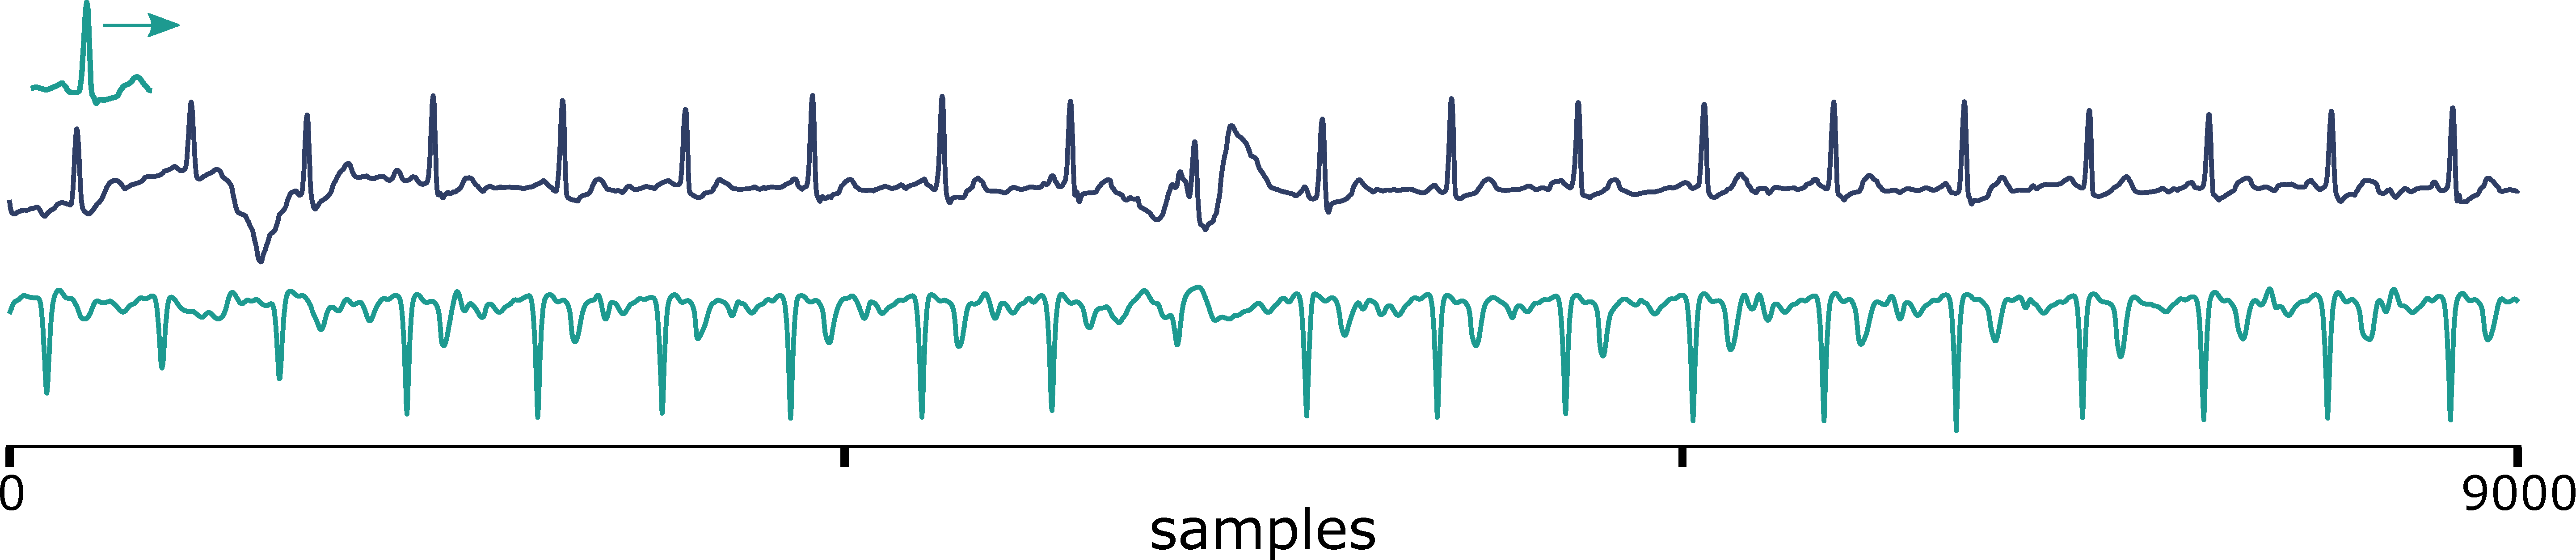
\includegraphics[width=\linewidth]{2_10_dist_profile_byquery.pdf}
\caption{Distance profile of a query based search using the z-normalized \gls{ed}. The template was a PQRS complex of an ECG.}
\label{fig:query_based}
\end{figure}

Other methods can be used to perform query-based search tasks, even using other types of templates, which can be a \textit{drawing} \cite{qetch} or text \cite{text_query1}. In this work, we will introduce novel ways of performing a query-based search with \gls{regex} and natural language.

\subsection{The k-Nearest Neighbors}

Having distance measures we can compare signals for several purposes, namely classification. One traditional supervised algorithm for this purpose is the k-\gls{nn}. The assumption of this method is fairly straightforward: new examples will be classified based on the class of their \gls{nn}, that is, the class of the example is the average of the class of its k-\gls{nn}. The process has two steps: (1) finding the k-\gls{nn} and (2) choosing the class of the example based on the neighbors \cite{knn}.
\par
In order to find the \gls{nn}, the distance from the example to all the time series of the training set has to be computed. The k-\gls{nn} are the $k$ training examples with the lowest distance. Having the \gls{nn}, the next stage is the determination of the example's class, which can be made with several strategies, such as majority voting, or distance-weighted voting \cite{knn}.
\par
In this work, we will propose a novel method for time series classification that will have its performance compared with a 1-\gls{nn} based on the z-normalized \gls{ed}. The proposed method is from the text-domain. As we have been mentioning in this manuscript, parts of the work developed are tightly connected with text mining methods by making a bridge between time series and text. It is then relevant to explain this relationship and how we can use it for time series data mining applications. 

\section{Text Mining on Time Series}
\label{sec:text_time}

%The representation of a time series into the symbolic domain makes possible the usage of text mining methods to analise time series. The reader will appreciate that an association regarding time series and text is made, and are also introduced relevant methods as the text mining domain, used in this work.

\subsection{Time Series Textual Abstraction}
\label{subsec:text_abstraction}

In \gls{sax} (see Section \ref{subsec:sax}), the signal is transformed into a sequence of symbols. For this, each sample of the \gls{paa} representation is converted into a \textit{character}, which can then form \textit{words} and \textit{sentences}. As a novel symbolic representation of time series is proposed in this work, it is relevant to give the general background that helps make the association between the original time series, how it can be transformed into a symbolic time series, and the text notation that can be used for this purpose. Note that this is an introductory explanation that will be further contextualized when needed throughout this manuscript. We start with fundamental definitions.\\\\
\textbf{Character:} A \textit{character}, $c$, is an unit symbolic element belonging to the vocabulary $V$ that represents a sample or \textit{subsequence} of a time series, such that $c \in V$. Each sample of a time series is transformed into a \textit{character} to form a \textit{symbolic time series}.\\\\
\textbf{Symbolic Time Series:} A \textit{symbolic time series} is a sequence of \textit{characters} ordered in time generated from the parent time series. It has length $n \in \mathbb{N}$: $ST = (st_1, st_2, ..., st_n)$, with $st_i = c \in V$. A specific sequence of \textit{characters} of a \textit{symbolic time series} can form a \textit{word}.\\\\
\textbf{Word:} A \textit{word} can be a single character or the concatenation of a sequence of \textit{characters}, giving a textual representation of a \textit{subsequence}, such that $W = (w_1, w_2, ..., w_u)$, with $u \in \mathbb{N}$, $w_i = c \in V$ and $W \in V$. Putting \textit{words} together forms a \textit{sentence}.\\\\
\textbf{Sentence:} A \textit{sentence} $S$ represents a group of \textit{subsequences} of the time series, or the entire time series itself. It is formed by joining sequences of \textit{words}, such that $S = W_1, W_2, ..., W_s)$, with $s \in \mathbb{N}$ and $W_i \in V$.\\\\
\textbf{Document:} The set of \textit{sentences} in a time series are called a \textit{document}. The \textit{document} $D$ can be computed by one or more sentences. In this work, a \textit{document} represents the textual description of the entire time series.\\\\
\textbf{Corpus:} The \textit{corpus} is a collection of text material (group of \textit{documents}). It represents a higher level of textual information that is used in case we have a dataset with multiple time series. This collection is typically annotated and used for machine learning tasks. In this case, a corpus will be represented by the set of \textit{documents} that describe an entire time series dataset.\\\\
\textbf{Vocabulary:} The \textit{vocabulary} $V$ comprehends the set of all different \textit{characters} and \textit{words} present in all time series of the dataset.\\

\subsection{Text Features}
\label{subsec:text_features}

Here are introduced traditional methods applied for feature extraction of text data, namely the \gls{bow} and  \gls{tfidf}.\\\\
\textbf{Bag of Words:} A \gls{bow} is a feature matrix representation of a corpus, being the feature the number of occurrences of each \textit{term} (in this case it can be a \textit{character} or a \textit{word}), called the \gls{tf}:
\begin{equation}
\label{eq:tf}
    bow(t,d) = tf_{t, d} = \frac{f_{t,d}}{\sum\limits_{t'\in d} f_{t',d}}, 
\end{equation}

being \textit{t} the term that exists in a document, \textit{d} the document and \textit{t'} the term that belongs to document \textit{d}. Here $t$ can be a single \textit{word} or an \textit{n-gram}.\\\\
\textbf{N-gram:} It is a span of followed \textit{words} that are counted in the \gls{bow}/\gls{tfidf}. As an example, a possible \textit{2-gram} from Figure \ref{fig:sax} would be \texttt{aa}, \texttt{ca} or \texttt{ac}. This strategy resembles a \textit{moving window} with total overlap on time series, but for text. It can make the \gls{bow}/\gls{tfidf} model more robust since it relies in more than single \textit{word} statistics. It also has a very good fit for time series, considering that it can take into account time dependencies between \textit{words}, which reflects the time dependency seen in time series between \textit{subsequences} (e.g. it might be more meaningful to say that a signal has a \texttt{peak} next to a \texttt{valley} than just saying that it has a \texttt{peak} and a \texttt{valley}).\\

The \gls{bow} is commonly used to vectorize the textual representation of each symbolic time series, but there is common knowledge in the text mining community that if a \textit{term} occurs in all \textit{documents}, then it is less relevant. In order to counteract this possible limitation, the \gls{tfidf} matrix is used.\\\\
\textbf{Term Frequency Inverse Document Frequency:} The \gls{tfidf} matrix increases the relevance of $t$ by means of the $t_f$, while reducing its importance in proportion to the number of \textit{documents}, $d$ that contain the term $t$. The model is defined by being a ratio between the $t_f$ and the \textit{inverse document frequency} (idf), which is calculated as follows:

\begin{equation}
\label{eq:idf}
    idf(t, D) = \log{\frac{L}{|\{d \in D: t \in d|\}}}
\end{equation}

\textit{L} is the total number of documents ($L = |D|$). The final equation of the \textit{tfidf} model is the following:

\begin{equation}
\label{eqn:tfidf}
    tfidf(t, d, D) = tf(t, d) \cdot idf(t, D) 
\end{equation}

Both \gls{bow} and \gls{tfidf} are matrices that have a vector representation of each \textit{document}, where each element of the vector is the relevance of the \textit{term}. That means that the euclidean or cosine distance (among others) can be used to compute the difference between \textit{documents}.
\par
Due to the probabilistic nature of the \gls{bow} and the fact that it contains discrete features, it is suitable to use in naïve Bayes classifiers. In the other end, the \gls{tfidf} is typically used with linear \gls{svm} classifiers \cite{scikit-learn}.

\subsection{Text-based Classifiers}
\label{subsec:text_classifiers}

As mentioned in the previous Section, linear classifiers, such as naïve Bayes and \gls{svm}s, are conventionally used for text document classifications. We will briefly explain the mechanisms of each of these classifiers that will be used in this work.

\subsubsection{Naïve Bayes Classifier}
\label{subsec:bayesian}

Naïve Bayes classifiers are a set of probabilistic linear classifiers that follow Bayes' theorem \cite{bayes_rule, NB_site}, which implies that the probability of an event occurring is based on \textit{prior} knowledge of conditions that might be related with this event. The term \textit{naïve} is used because these classifiers assume that features are mutually independent. 

The probability of an event translates as the probability of an object belonging to a specific class ($w_j$) given the observed features ($x_i$ - feature vector). This probability ($P(w_j|x_i)$ - posterior probability) is given by the general equation based from Bayes' theorem \cite{bayes_rule, NB, NB_site}:

\begin{equation}
P(w_j|x_i) = \frac{P(x_i|w_j) \dot P(w_j)}{P(x_i)}.
\end{equation}

\begin{itemize}
\item $P(x|w_j)$ is the class-conditional probability (likelihood), which calculates \textit{how likely} the feature is observed given that it belongs to class $w_j$. It includes the probabilistic contributions of all feature dimensions:

\begin{equation}
P(x|w_j) = P(x_1|w_j) \dot P(x_2|w_j) ... \dot P(x_n|w_j) = \prod^n_{k=1}P(x_k|w_j)
\end{equation}

\item $P(w_j)$ is the \textit{prior probability}. The general probability of a class. In case the classes are uniformly distributed, the posterior probability is dependent on the class-conditional probabilities.
\item $P(x)$ is the \textit{evidence}, which is the probability of encountering feature $x$ independently of the class label.
\end{itemize}

During the training process, the posterior probability is maximized. Several approaches can be found to compute naïve Bayes models, namely \textit{Gaussian}, \textit{Multinomial}, \textit{Complement}, \textit{Bernoulli} and \textit{Categorical} naïve Bayes. In this manuscript, we will show the usage of a \textit{Multinomial} naïve Bayes model for classification, which uses word count feature vectors and is more appropriate to be used with \gls{bow} or \gls{tfidf} models. We will use the \textit{Python} implementation given by the \textit{scikit-learn} package called \textit{MultinomialNB} \cite{scikit-learn}.

\subsubsection{Linear Support Vector Machines (SVM)}
\label{subsec:svm}

The \gls{svm} classifier is a conventional method that separates different classes by finding the \textit{hyperplane} from $n$-dimensional space ($n$ equal to the number of features) that puts all samples from the same class the furthest apart from the other classes' samples. The training process has the purpose of finding this hyperplane by maximizing the margin distances between the hyperplane's surface and all samples. The hyperplanes can be written as the set of features $x$ that satisfy the following equation: 

\begin{equation}
\mathbf {w} ^{\mathsf {T}}\mathbf {x} - b = 0,
\end{equation}

where $\mathbf {w}$ are the weights for the optimal hyperplane, given as a linear combination of support vectors \cite{svm}. The support vectors belong to samples that give shape and orientation to the hyperplane. There are several ways of performing the maximum-margin hyperplane optimization, originally linear, but with non-linear metrics also available. In this work, we used the linear \gls{svm} implementation available at the \textit{Python} implementation given by the \textit{scikit-learn} package called \textit{LinearSVC} \cite{scikit-learn}.

\subsection{Text Pattern Search}
\label{subsec:regex_theory}

When writing or reading a document, we often use shortcuts or other commands to speed up the task of searching for specific words or expressions. In some cases, we might not be searching specifically for a character or word, but rather for a text structure or text pattern (for example, one might be searching for all the emails available in a text document). This type of search is comparable to querying in time series, being the most convenient method to perform this type of search in text a \gls{regex}.
\par
A \gls{regex} is a parsing technique that is convenient to write text patterns, being more flexible than direct matches. It is based on regular languages, follows a specific set of rules, and contains a set of meta-characters.
\par
In order to understand the way that \gls{regex} work, some of the most used characters and \gls{regex} primitives are presented as follows \cite{regex2}:

\begin{table}[!h]
\centering
\renewcommand{\arraystretch}{1.25}
\begin{tabular}{ABC}
\toprule
\textbf{MC} & \textbf{Description} & \textbf{Example of Match}\\
\midrule
\textbf{*} & The preceding item will be matched zero or more times & \textit{eve*nt} $\rightarrow$ [evnt, event, eveent]\\

\textbf{+} & The preceding item will be matched one or more times & \textit{su+b} $\rightarrow$ [sub, suub, suuub]\\

\textbf{?} & The preceding item is optional and will be matched, at most, once & \textit{team?}$\rightarrow$ [tea, team]\\

\textbf{.} & Matches any character & \textit{s.m} $\rightarrow$ [ssm, sam, sim] \\

\textbf{[]} & Matches anything inside the brackets & \textit{wom[ae]n} $\rightarrow$ [women, woman] \\

\textbf{|, \&} & Boolean operators - or, and & \textit{tr(i|a)p} $\rightarrow$ [trip, trap]\\

\textbf{(?=<)} & Positive lookbehind - The string matches the item that is preceded by the pattern inside the lookbehind without making it part of the match & \textit{(?=<http://)} $\rightarrow$ any URL\\

\textbf{(?<!)} & Negative lookbehind - The string matches the item that is not preceded by the pattern inside the lookbehind & \textit{?<!$\backslash$ d*}.+ $\rightarrow$ [\cancel{10th}, th]\\

\textbf{(?=)} & Positive lookahead - The string matches the preceding item that is followed by the pattern inside the lookahead without making it part of the match & \textit{(?=www$\backslash$ .)} $\rightarrow$ matches web protocol\\

\textbf{(?!)} & Negative lookahead - The string matches the preceding item that is not followed by the pattern inside the lookahead & a(?!b) $\rightarrow$ [\cancel{ab}, ac]\\
\bottomrule
\end{tabular}
\caption{Main \gls{regex} operators and meta-characters. Each is presented with a simple example of a good match for a possible \gls{regex}. A description is also made for complementary understanding.}
\label{tab:regex}
\end{table}

%\subsection{Keyword Extraction}
%
%https://www.analyticsvidhya.com/blog/2018/11/introduction-text-summarization-textrank-python/


\section{Performance and Validation Measures}

This manuscript discusses three main time series data mining problems, namely classification, segmentation, and event/pattern detection. In order to perform a validation of the work developed, standard procedures are used. In this section are explained which procedures are typically employed to evaluate the performance of algorithms in the mentioned problems.

\subsection{Classification Problems}

One of the most common strategies to evaluate algorithms from the machine learning field are \textit{precision} (P), \textit{recall} (R) and \textit{f1-score} (F1). These measures are calculated based on \textit{true positives} (TP), \textit{false positives} (FP) and \textit{false negatives} (FN). Understanding what these metrics represent depends on the problem. These measures are used in this thesis to evaluate the performance of classification and event detection algorithms.

In time series classification problems, a labeled dataset is divided into training and testing sets. The algorithm learns on the training set and a final evaluation is made on the testing set. In case the algorithm needs to fine-tune \textit{hyperparameters}, it is good practice to perform a cross-validation during the training stage. This ensures that the algorithm is optimized without \textit{seeing} any testing samples and prevents \textit{overfitting}. Several strategies can be used to perform the separation of the training set, such as the \textit{k-fold} or \textit{leave one out}. Besides, these can be made by shuffling, stratifying or grouping it. Choosing the most adequate cross-validation method depends on the distribution of the training samples.

In order to perform the validation or final evaluation of the algorithm, the ground truth labels are compared with the labels predicted by the algorithm on the testing set. This comparison gives the number of \textit{TP}, \textit{TN}, \textit{FP} and \textit{FN}.

\begin{itemize}
    \item $TP_c$ - If the label predicted by the algorithm is equal to the target class (positive when positive);
    
    \item $TN_c$ - If the label predicted is correctly not the target class (negative when negative).

    \item $FP_c$ - If the label predicted by the algorithm is falsely classified as the target class when it should not (positive when negative);
    
    \item $FN_c$ - If the label predicted by the algorithm is not labeled as the target class when it should (negative when positive).
    
\end{itemize}


\begin{equation}
\label{eq:precision}
Precision (P) = \frac{TP}{TP+FP}
\end{equation}

\begin{equation}
\label{eq:recall}
Recall (R) = \frac{TP}{TP+FN}
\end{equation}

\begin{equation}
\label{eq:f1_score}
F1-score (F1) = 2 \times \frac{P*R}{P+R}
\end{equation}

\begin{equation}
\label{eq:accuracy}
Accuracy (A) = \frac{TN+TP}{TN+TP+FP+FN}
\end{equation}

These measures were initially performed in binary classification problems, but can be adapted in multi-class ones as well. For this, each class (the target class) is compared to all the other classes, being the target class the \textit{positive} and all the other classes \textit{negative}. All measures are calculated for each class, and a macro and micro average of these metrics are finally calculated (here $c$ represents the number of classes).

\begin{equation}
macroP = \Sigma_{i=0}^c \frac{P_i}{c}
\end{equation}

\begin{equation}
macroR = \Sigma_{i=0}^c \frac{R_i}{c}
\end{equation}

\begin{equation}
microP = \frac{\Sigma_{i=0}^c TP_i}{\Sigma_{i=0}^c TP_i + \Sigma_{i=0}^c FP_i}
\end{equation}

\begin{equation}
microR = \frac{\Sigma_{i=0}^c TP_i}{\Sigma_{i=0}^c TP_i + \Sigma_{i=0}^c FN_i}
\end{equation}

These metrics are typically supported with a \textit{confusion matrix}, which displays a 2D-map of the ground truth labels \textit{versus} predicted labels.

\subsection{Event Detection}
\label{subsec:event_metrics}

Regarding event detection problems, the process involves finding the sample that corresponds to the ground truth event. Considering that it would not be fair to calculate the performance of an event detection algorithm only by searching if the ground truth sample exactly matches the ground truth, we calculate the \textit{TP}, \textit{FP} and \textit{FN} based on a tolerance margin. From these measures, metrics from Equations \ref{eq:precision}, \ref{eq:recall} and \ref{eq:f1_score} are calculated. The estimated events are considered one of the following categories:

\begin{itemize}
    \item $TP_e$ - is counted when the estimated event is in the margin around the ground-truth event;
    
    \item $FP_e$ - is counted whenever it is out of a margin around the ground-truth event, or when there is more than one estimated event inside the margin;
    
    \item $FN_e$ - is counted when there is no estimated event inside the margin of the ground-truth events.
    
\end{itemize}

Additionally, the distance of the \textit{TP} events from the ground-truth events can be calculated with the \gls{mae}:

\begin{equation}
    MAE = \sum^{k}_{i=1} \frac{|g_{i} - e_{i}|}{k}
\end{equation}

%
%\begin{equation}
%    MSE = \frac{1}{k} \sum^{k}_{i=1} (g_{i} - e_{i})^2
%\end{equation}
%
%\begin{equation}
%    ME = \frac{1}{k} \sum^{k}_{i=1} (g_{i} - e_{i})
%\end{equation}

The precision measure is relevant to indicate if the method can only estimate events that belong to the ground-truth category, while the recall measure is an important indication of how many ground-truth events are missed in the estimation of the method. Both measures are combined in the F1-measure.


%\par
%The distance-based metrics evaluate how far are the TP from the corresponding ground-truth events (\gls{mae} and \gls{mse}) and which is the direction of estimation of events (if before or after the ground-truth events - \gls{Mse}).

\subsection{Evaluating Query Complexity}
\label{subsec:complex}

As we are introducing novel ways of performing more expressive query-based searches with \gls{regex}, we are measuring the legibility and difficulty in generating a query. In the programming field, \textit{Halstead} measures are typically used for this purpose. These measures describe the complexity of the script directly from the source code, based on a set of metrics calculated with the number of distinct \gls{oprt} and \gls{oprd}, and the \gls{Toprt} and \gls{Toprd}. These metrics are the \cite{Halstead2}:

\begin{description}
 	\item [\textbf{Vocabulary}] 
    	The number of distinct operators and operands that belong to the script:
        \begin{equation}
        \centering
        Voc = \gls{oprt} + \gls{oprd}
        \end{equation}
    
     \item [\textbf{Length}] \hfill \\
    	The total number of operators and operands that belong to the script:
        \begin{equation}
        	\centering
        	Lgth = \gls{Toprt} + \gls{Toprd}
        \end{equation}
        
     \item [\textbf{Calculated Length}] \hfill \\
    	It uses the entropy measure to calculate the average amount of information based on the number of distinct operators and operands:
        \begin{equation}
        	\centering
        	CL = \gls{oprt}*\log_2(\gls{oprt}) + \gls{oprd}*\log_2(\gls{oprd})
        \end{equation}
       
     \item [\textbf{Volume}] \hfill \\
    	It measures the amount of information that the reader has to absorb to understand its meaning. It is proportional to the length measure ($Lgth$) and logarithmically increases with the vocabulary:
        \begin{equation}
        	\centering
            Vol = Lgth*\log_2(Voc)
        \end{equation}
        
     \item [\textbf{Difficulty}] \hfill \\
    	The difficulty in writing or reading the script. It increases more having fewer operands repeated more frequently than having more operands repeated more frequently:
        \begin{equation}
        	\centering
            Dif = (\frac{\gls{oprt}}{2} + \frac{\gls{Toprd}}{\gls{oprd}})
        \end{equation}
        
	 \item [\textbf{Effort}] \hfill \\
    	Measure of the effort necessary to understand what is written and recreate the script. It is proportional to both volume and difficulty measures:
        \begin{equation}
        	\centering
        	Efrt = Vol*Dif
        \end{equation}
\end{description}


\subsection{Comparing Algorithms' Performances}

In science, a good practice is to compare the proposed algorithm with other existing solutions, such that the reader can understand how the results presented are unbiased from the data. In this work, each strategy proposed in the domains of classification and event detection will be compared with existing solutions. Typically, the results will have accuracy or F1-scores metrics, sometimes from very large datasets. Averaging these scores may not give a reliable view of performance differences between methods, specially if these scores are the performance of the algorithm over different datasets, with different sizes, scenarios and difficulties. In that case, other techniques should be used to present the results such that the reader can have the full picture. 

One possible strategy involves counting the times a method wins, draws or loses against another method. This can be helpful to have a broader picture of the results in addition to the average metrics. We will use this count strategy for both classification and segmentation tasks since we will be using multiple datasets, with different lengths, difficulties and contexts. 

Visual tools can also be employed for this purpose, namely \textit{confrontation maps} and \textit{critical distance maps}, with examples displayed on Figures \ref{fig:performance_plots}.left and \ref{fig:performance_plots}.right, respectively.

\begin{figure}
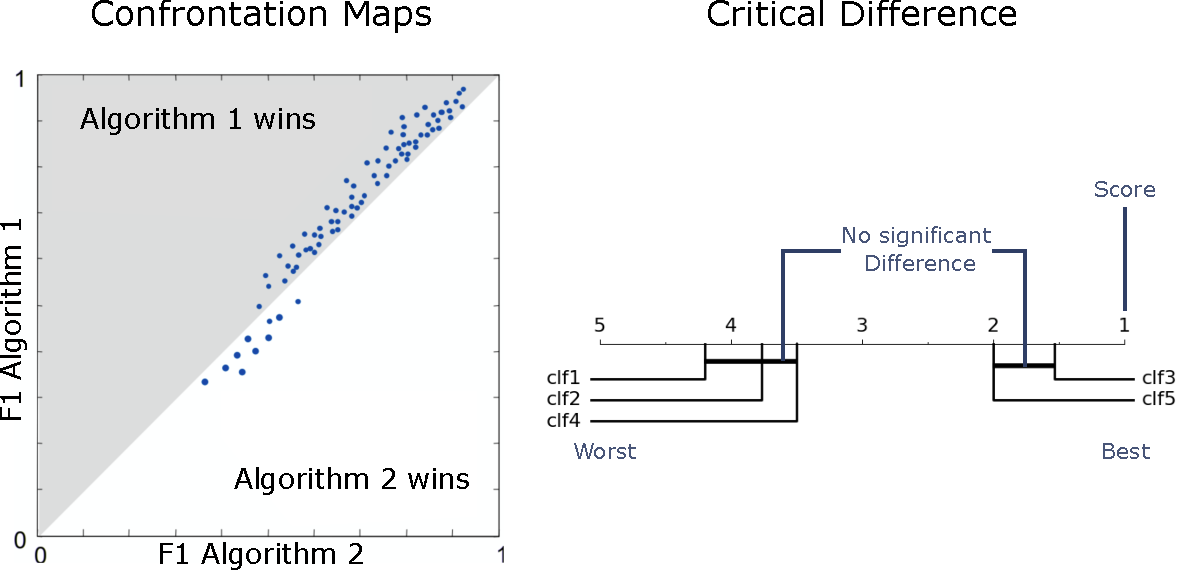
\includegraphics[width=\linewidth]{performance_plots.pdf}
\caption{On the left are confrontation maps, used to compare classification algorithm performances. On the right is a critical difference map, which shows a statistical difference in the performance of algorithms for general purposes.}
\label{fig:performance_plots}
\end{figure}

\subsubsection{Confrontation Maps}
\label{sec:maps1}

When the proposed algorithm is applied to a dataset and compared with another algorithm, we might be tempted to display an overwhelming quantity of information in a table. Although this is a valid approach that should be made to give a full picture to the reader, there should also be a straightforward way of displaying the same information, but reading it at a glance. With confrontation maps, we can compare the performance of two algorithms just to very intuitively understand if there is a significant difference in their performance. Typically, this map is a scatter plot comparing the \textit{F1-score} or \textit{accuracy} of algorithm 1 \textit{versus} algorithm 2. Figure \ref{fig:performance_plots}.left displays an example of it taken from \cite{keogh_presentation}. Each dot of the plot is a dataset. When it is above the diagonal, it is better classified by algorithm 1, while if below, it is better classified by algorithm 2. In this example, algorithm 1 is better in most datasets.

\subsubsection{Critical Distance}

Critical distance maps are a way of comparing the performance of multiple algorithms or variations of the same algorithm. The plot is a representation of a statistical test over the performance result of each algorithm. The test evaluates if the difference in the performance is significant (critical distance) or not. For instance, in Figure \ref{fig:performance_plots}.right, the plot compares five different classifiers (\textit{clf1} to \textit{clf5}) and highlights that the difference in performance is not significant between \textit{clf1, 2} and \textit{4}, neither between \textit{clf3 and 5}. However, \textit{clf3} and \textit{5} have a much better performance than the other classifiers. The closer the classifiers are from the right (1), the better they are. The tick bar connects the classifier with performances that are not significantly different in the statistical test.
\par
This method receives the performance scores (such as F1-scores, accuracies, etc...) of multiple classifiers. This type of comparison gives a more appropriate explanation of the differences between different methods than a simple average. This is even more relevant in cases where the methods are applied in multiple datasets that have different size, lengths, and/or difficulty, and where the average performance results would be not fair to describe the differences.
\par
In this work, we will use an implemented critical distance method from \cite{critical_dif}, which uses the  \textit{Wilcoxon-Holm} test to counteracts the problem of multiple comparisons and calculates pairwise significance between all methods evaluated \cite{stat_test}. The null hypothesis of the \textit{Wilcoxon} signed rank test is that the median of the population of differences between the paired data is zero, while the alternative hypothesis is that it is not. The significance is then evaluated with the \textit{Holm} test to accept or reject the multiple hypothesis results based on the p-values resulting from the pairwise tests.